% biber main
% pdflatex main.tex

\documentclass{report} %article or report
\usepackage{nameref} % to get the name of the section to reference
\usepackage{hyperref} % hyperlinks to references
\usepackage{graphicx} % Required for inserting images
\usepackage{xcolor} % For text colors
\usepackage{wrapfig}  % to wrap text around images
\usepackage[rightcaption]{sidecap}  % caption to the side of the image
% \usepackage{svg} % for .svg images
\usepackage{subfig} % for more figures together
\usepackage{amsmath} % math things ?
\usepackage[skip=10pt plus1pt, indent=0pt]{parskip}
\usepackage{titlesec} % improve chapter titles
% \usepackage{todonotes} % adds notes to the side, actually these slow down the compilation by a ton
\usepackage{tabularx}
% \usepackage{rotating}   % rotating tables? 
\usepackage{lscape}    % rotating tables????
% \usepackage{adjustbox}  % I use it to rotate a table
\usepackage{makecell}  % to make two line elemenents in a cell
\usepackage[symbol]{footmisc} % to use symbols for footnotes (https://tex.stackexchange.com/questions/826/symbols-instead-of-numbers-as-footnote-markers)
\usepackage{siunitx}  % SI units
\usepackage[backend=biber, sorting=none, maxnames=2, style=nature]{biblatex} %Imports biblatex package
\usepackage{xcolor} % For text colors
\usepackage{tablefootnote}  % footnotes in tables don't appear otherwise

% \usepackage{biblatex} %Imports biblatex package
%THIS TO INCLUDE THE VAVILOV_LANDAU LATEX FILE
% \usepackage{Vavilov_packages}

% \newcommand{\specialcell}[2][c]{%
%   \begin{tabular}[#1]{@{}c@{}}#2\end{tabular}}

\hypersetup{
    colorlinks,
    citecolor=black,
    filecolor=black,
    linkcolor=black,
    urlcolor=black
}

\addbibresource{bibliography.bib} %Import the bibliography file

\title{TestBeam analysis for HGTD}
\author{Marcello Pozzessere}
\date{January 2025}

\begin{document}

\maketitle
% \renewcommand{\thesection}{\arabic{section}}
% \titleformat{\chapter}{\bfseries\huge}{\thechapter.}{20pt}{\huge\it}
\titleformat{\chapter}[hang]{\Huge\bfseries}{\thechapter\,\textcolor{gray}{|}\,}{0pt}{\Huge\bfseries}

\tableofcontents

%%% intro on LHC 
%%% ATLAS and HGTD
%%% 

\chapter{Introduction}

\section{The LHC and the High Luminosity upgrade}

The Large Hadron Collider (LHC)is the largest particle accelerator in the world. Built between 1998 and 2008 by the European Organization for Nuclear Research (CERN, \textit{Conseil européen pour la Recherche nucléaire}) in collaboration with more than 100 countries. 
It achieved beam energies of more than 6.5 TeV and enabled many historic discoveries in particle physics.
Along the accelerator track there are four main experiments: ALICE, ATLAS, CMS, LHCb (Figure \ref{fig:LHC}). 

\begin{figure}[!h]
    \centering
    \includegraphics[width=.8\textwidth]{Images/intro/LHC.png}
    \caption{LHC scheme and the four main experiments. Each particle (typically proton or lead ion) is accelerated from the Proton Synchrotron into the Super Proton Synchrotron and finally into the Large Hadron Collider}
    \label{fig:LHC}
\end{figure}


The High-Luminosity phase of the Large Hadron Collider (HL-LHC), which should be operational in 2029 \cite{LS3_schedule_change}, aims to increase the integrated luminosity by a factor of 10 \cite{CERN-LHCC-2020-007}.
This will give great opportunities for new physics but it will also introduce a wide range of new challenges.

% this is already kinda talking about HGTD, maybe it's a good bridge to the next section: HGTD


\section{The ATLAS experiment and the HGTD}

ATLAS (\textbf{A} \textbf{T}oroidal \textbf{L}HC \textbf{A}pparatu\textbf{S}) is a general purpose detector built for probing \textit{p-p} and \textit{A-A} collisions (\textit{proton-proton} and \textit{heavy ion-heavy ion}, respectively). \marginpar{\flushleft can be improved}
The experiment's main components are: Inner Detector, Calorimeters and Muon Spectrometer \cite{Collaboration_The_ATLAS2008}.

\begin{figure}[!h]
    \centering
    \includegraphics[width=\textwidth]{Images/intro/ATLAS_with_description.jpg}
    \caption{ATLAS experiment and its main components}
    \label{fig:ATLAS}
\end{figure}

A considerable challenge that will arise with the High Luminosity upgrade will be the increase of pile-up of events, i.e. collisions that will happen too close to each other to be individually resolved. 
A new way to mitigate this effect will be "\textit{to use high-precision timing information to distinguish between collisions occurring very close in space but well-separated in time}" \cite{CERN-LHCC-2020-007}. This is set to be accomplished by the High Granularity Time Detector (HGTD).

% picture of HGTD
\begin{figure}
    \centering
    \subfloat[Location]{
        \includegraphics[width=.6\textwidth]{Images/intro/HGTD position and layout.jpg}
        \label{fig:HGTD_location}}
    \hfill
    \centering
    \subfloat[Schema]{
        \includegraphics[width=.35\textwidth]{Images/intro/HGTD_schema.jpg}
        \label{fig:HGTD_schema}}
    \caption{Location and schema of the HGTD inside ATLAS}
\end{figure}

% eta=2.4 -> theta=10.367°      eta=4 -> theta=2.0986°
The detector will cover pseudrapidities between $2.4 < \eta < 4.0$ \footnote{the pseudorapity is $\eta=-\ln \tan(\theta/2)$ where $\theta$ is the polar angle from the $z$ axis, i.e. the beam direction.} (so an incident angle roughly between 2° and 10°), complementing the ITk (Inner Tracker) which has worse resolution in this forward region. The luminous region in the nominal scenario for Run 3 will see a Gaussian spread of approximately 50mm along the $z$ axis and a width of 175$\si{ps}$ in time (Figure \ref{fig:events_pileup}). HGTD will provide time information of charged particles with a time resolution of 30ps (up to 50ps at the end of life) which will greatly improve the reconstruction of the primary vertex of collision.


\begin{figure}[!hb]
    \centering
    \includegraphics[width=.8\textwidth]{Images/intro/events_pileup_HL_LHC.jpg}
    \caption{Visualization of the pile-up of events inside ATLAS, using simulation data (PUT SOURCE AND MORE EXPLANATIONS (what is HS?))}
    \label{fig:events_pileup}
\end{figure}


%%% what LGADs are
%%% working principles
%%% requirements for the detector
%%% other studies 
%%% expected results
\chapter{LGADs} 

\marginpar{\flushleft Add other image/photo of LGAD}

\section{Working principles of silicon sensors}

The core of a silicon sensor consists of a junction between two differently doped layers, which means that small concentrations of impurities with either higher atomic number ($n$-type) or lower ($p$-type) are introduced inside the crystals.
This forms a $pn$-junction and when a voltage is applied with positive potential on the $n$-side and negative on the $p$-side (reverse bias) the volume between the two layers is depleted of mobile charges and becomes an insulator with an internal electric field.

% %%% FIGURE WITH SIDE CAPTION
% \sidecaptionvpos{figure}{c}
% \begin{SCfigure}
%     \includegraphics[width=.4\linewidth]{Images/LGADs/p-n junction with voltage.png}
%     \caption{Top: adjacent regions of $p$-doping (left) and $n$-doping forming a $pn$-junction. Middle: the circled mobile charges (holes for $p$-type and electrons for $n$-type) balanced by the charge of atomic cores. Bottom: When an external (reverse) voltage is applied to the central region an electric field builds up in the junction.}
% \end{SCfigure}

%%% WRAPPED FIGURE
% \begin{wrapfigure}{l}{.45\linewidth}
%     \includegraphics[width=1\linewidth]{Images/LGADs/p-n junction with voltage.png}
%     \caption{Top: adjacent regions of $p$-doping (left) and $n$-doping forming a $pn$-junction. Middle: the circled mobile charges (holes for $p$-type and electrons for $n$-type) balanced by the charge of atomic cores. Bottom: When an external (reverse) voltage is applied to the central region an electric field builds up in the junction.}
%     \label{fig:p-n_junction_reverse_bias_voltage}
% \end{wrapfigure}

%%% FIGURE WITH MINIPAGE
\begin{figure}[!h]
    \begin{minipage}[c]{.25\linewidth}
        \includegraphics[width=1\linewidth]{Images/LGADs/p-n junction with voltage.png}
    \end{minipage}
    \hfill
    \begin{minipage}[c]{.6\linewidth}
        \caption{\\Top: adjacent regions of $p$-doping (left) and $n$-doping (right) forming a $pn$-junction.\\
        Middle: the circled mobile charges (holes for $p$-type and electrons for $n$-type) balanced by the charge of atomic cores.\\
        Bottom: When an external (reverse) voltage is applied to the junction an electric field builds up in the central region \cite{10.1093/acprof:oso/9780198527848.003.0001}.}
    \end{minipage}
    \label{fig:p-n_junction_reverse_bias_voltage}
\end{figure} 

When a charged particle traverses this depletion layer it frees up electron-hole pairs, which move to the electrodes and can be measured. 

\section{Low Gain Avalanche Detectors}

A particular type of silicon sensors are Low Gain Avalanche Detectors (LGAD), an example is shown is shown in Figure \ref{fig:LGADs_schema}. The major innovation is an additional $p$-type layer below the $n+$ electrode, this creates a high electric field region which leads to an avalanche effect\footnote[2]{When electrons acquire enough energy they can create new electron-hole pairs ('impact ionization'), which can themselves create new pairs and initialize a multiplication chain that leads to an enhanced signal} of the electrons. This effect produces a gain of around $~10$ \marginpar{\flushleft source} 

\begin{figure}[!ht]
    \centering
    \includegraphics[width=.9\linewidth]{Images/LGADs/1-s2.0-S0168900214007128-gr1_lrg.jpg}
    \caption{description of LGAD}
    \label{fig:LGADs_schema}
\end{figure}

\section{The sensors}
There were several samples that were tested, divided into three main categories of design:
\begin{itemize}
    \item USTC, from the University of Science and Technology of China
    \item IHEP, from the Institute of High Energy Physics, China
    \item CNM, from the Centro National de Microelectronica, Barcelona, Spain
\end{itemize}

the first two designs have both been manufactured by the IME (Institute of Microelectronics) of the Chinese Academy of Sciences. The two CNM sensors (labeled CNM-W4 and CNM-W5) were used to measure the time resolution of another device, the MCP (Section \ref{sec:MCP_description}), which was used as a time reference for all of the time measurements of the other LGADs. Table \ref{tab:devices_tested} provides the list of the devices that were characterized, for more detailed descriptions see Table in \nameref{chap:appendix}.

\begin{table}[!ht]
    \centering
    \caption{Summary of the tested devices}
    \label{tab:devices_tested}
    \scriptsize
    % \makebox[1\textwidth][c]{
    \begin{tabularx}{1\textwidth}{|l|l|l|l|l|X|}
    \hline %%% I NEED TO TRY TO USE TABULAR INSTEAD OF SHORTSTACK
        \textbf{Sevice name} & \textbf{Vendor} & \begin{tabular}{@{}l@{}}\textbf{Pads,} \\ \textbf{used channels}\end{tabular} & \begin{tabular}{@{}l@{}}\textbf{Fluence} \\ $[n_{eq}/\si{cm^2}]$ \end{tabular} & \begin{tabular}{@{}l@{}} \textbf{Radiation} \\ \textbf{type} \end{tabular} & \textbf{Notes} \\
        \hline
        CNM-W4  & CNM & single & 0 & - & reference \\ 
        CNM-W5  & CNM & single & 0 & - & reference \\ 
        CNM-W5-1.5E15  & CNM & single & $\num{1.50E+15}$ & neutron &  \\ 
        CNM-W3-2.5E15  & CNM & single & $\num{2.50E+15}$ & neutron &  \\ 
        USTC2.1-W17 & USTC & 2x2, 2 channels  & 0 & - &  \\ 
        USTC2.1-W17-2E14 & USTC & 2x2, 1 channel & 0 & - & missing \\ 
        IMEv3-W12-2x2  & IHEP & 2x2, 2 channels  & 0 & - &  \\ 
        IMEv3-W12-1x3  & IHEP & 1x3, 2 channels  & 0 & - &  \\ 
        IMEv3-W12  & IHEP & 2x2, 3 channels  & $\num{1.50E+15}$ & neutron &  \\ 
        IMEv3-W16  & IHEP & 1x3, 1 channel  & $\num{1.50E+15}$ & neutron &  \\ 
        IMEv2-W7-1E14  & IHEP & single & $\num{1.00E+14}$ & proton &  \\ 
        IMEv2-W7-6.5E14  & IHEP & single & $\num{6.50E+14}$ & proton &  \\ 
        IMEv3-W16-8E14  & IHEP & single & $\num{8.00E+14}$ & proton &  \\
        IMEv3-W16-2.5E15  & IHEP & single & $\num{2.50E+15}$ & neutron &  \\ 
        \hline
    \end{tabularx}
\end{table}




%%% NOT UPDATED ANYMORE, LOOK AT THE EXCEL FILE, I MIGHT DELETE THIS LATER
%%% I have to reorganize these and associate them with the more accurate descriptions
% device name:        vendor:        sensor ID:            fluence:    irradiation type:    type:        board name:    channels:
% CNM-W4              CNM          CNM-R15973-W4-D168      unirradiated      -             single pad     JSI-B12      1
% CNM-W5              CNM          CNM-R15973-W5-D138      unirradiated      -             single pad     JSI-B14      1
% CNM-W3-2.5E15       CNM          CNM-R15973-W3-D29       $\num{2.5e15}     neutron       single pad     JSI B5       1
% CNM-W5-1.5E15       CNM          CNM-R15973-W5-D29       $\num{1.5e15}     neutron       single pad     JSI PP1      1
% USTC2.1             USTC         USTC2.1-W17-P6-A          0                -             2x2           CERN-3       1,2
% USTC2.1 IRRADIATED (MISSING)
% IMEv3-W12-C2         IHEP        IMEv3-W12-C2-2-2          0               -              2x2          CERN-1       channels 1,2
% IMEv3-W12-C3         IHEP        IMEv3-W12-C3-1-4 (and 5)  0               -              1x3          CERN-1       channles 3,4  (small GR), bonded
% CERN2-CH0-IMEv3-W12  IHEP        IMEv3-W12-B2-2-9-1       1.5e15           neutron        2x2 sensor    CERN-2       channels 1,2,3
% CERN2-CH1-IMEv3-W12  IHEP 
% CERN2-CH2-IMEv3-W12  IHEP 
% CERN2-CH4-IMEv3-W16  IHEP        IMEv3-W16-Q4-D4-1-4      1.5e15           neutron        1x3          CERN-2       channel:  2(?)
% JSI-B6-IMEv2-W7-1E14    IHEP       W7-II-C2-1-7 IMEv2-W7Q2    1e14          proton        single       JSI-B6
% JSI-PP4-IMEv2-W7-6.5E14 IHEP       W7-II-C2-1-7 IMEv2-W7Q2    6.5e14        proton        single       JSI-PP4
% JSI-B7-IMEv3-W16-8E14   IHEP       IHEP-IMEv3-W16_Q4_D3_1-4   8e14          (unsure)        single       JSI-B7
% JSI-B13-IMEv3-W16-2.5E15 IHEP      IHEP-IMEv3-W16_Q4_E3_1-4   2.5e15       (unsure)      single        JSI-B13
                 

\chapter{Literature review}

I don't know about this, maybe I should just put very clear the requirements of the LGADS, HGTD and ALTIROC and that's it

\chapter{Test Beam setup}\label{chap:testbeam_setup}

%%% motivate testbeam
A typical way to test the performance of sensors for High-Energy Physics applications is with test beams: the Devices Under Test (DUTs) are put through a focused flux of high energy particles and their response is read out and analyzed. %%% aka testbeam

The HGTD collaboration has run many test beam campaigns, mainly at CERN and at DESY (Deutsches Elektronen-Synchrotron). The focus of this analysis is the test beam campaign of May 2023, conducted at CERN using a beam of \qty{120}{\giga\electronvolt} pions, provided by SPS.

\begin{figure}[h!tbp]
    \centering
    \includegraphics[width=.95\linewidth]{Images/TestBeam_setup/TestBeam_setup_redrawn.png}
    \captionsetup{width=\captionwidth}
    \caption{The main components of the test beam setup: the EUDET-type beam telescope with six MIMOSA planes, the FE-I4, the MCP and the cooling box containing the DUTs}
    \label{fig:testbeam_setup}
\end{figure}

The experimental setup of this campaign included:
\begin{itemize}
    \item FE-i4~\cite{Obermann:2014goa}: a hybrid pixel detector that provided a user-defined Region Of Interest (ROI), creating a HitOR\footnote{A binary signal generated when at least one pixel registers a hit} signal. %to avoid noisy pixels.
    \item Trigger Logic Unit (TLU): provided a trigger\footnote{A trigger is a signal that initiates data readout when a particle is detected}, combining the signals from a scintillator and the FE-i4. %% describe trigger??
    \item EUDET-type beam telescope equipped with 6 MIMOSA planes~\cite{Jansen:2016bkd}: used for precise spatial measurements of the particles in the beam, enabling track reconstruction.
    \item MicroChannel Plate detector (MCP)~\cite{LADISLASWIZA1979587}: measured the time of the moving particles, used as reference for the time resolution.
    \item Cooling box: contained the various DUTs, maintaining them at \qty{-30}{\degreeCelsius}.
    \item 2 oscilloscopes: acquired the data from the MCP and the DUTs. %%% I put later the channels
\end{itemize}

%%% maybe this should just be later

% description of components:
% • Trigger logic unit for particle passing
% • FEi4 to select a region of interest
% • Mimosa planes for tracking (X and Y position data)
% • MCP for time reference 
% • Cooling box containint the DUTs, (can be tilted with respect to the beam direction)
% • 120 GeV beam of pion

\section{TLU and FEi4}

The Trigger Logic Unit provided a trigger whenever a particle was detected. This trigger in turn instructed various components (in this case the oscilloscopes, the MIMOSA planes) to initiate data acquisition. More specifically the TLU took input from a scintillator and the FE-i4 to create a trigger.

The FE-i4 (Front-End-Iteration 4)~\cite{Obermann:2014goa} is a pixel readout chip with a planar silicon sensor bump bonded to it. It has a configurable sensitive area of up to \(\num{16.8} \times \qty{20}{\milli\meter^2}\) made up of 80 columns (\qty{250}{\micro\meter} pitch) and 336 rows (\qty{50}{\micro\meter}). 

Selecting a specific ROI allowed to exclude the areas outside the DUTs surface and to reduce sources of noise (e.g. noisy pixels of MIMOSA planes). %%% maybe the next part is just a repetition of what I say later
%It should be noted that in some occasions, due to erroneous ROI selection or due to small positional shifts caused by temperature fluctuations, the DUTs fell outside said ROI and the analysis was negatively impacted. (Example in Appendix, later)

\section{EUDET-type beam telescope}
A EUDET-type beam telescope~\cite{Jansen:2016bkd} equipped with a total of 6 Minimum Ionizing MOS Active Pixel Sensor planes~\cite{Hu-Guo:2010lrq} provided precise spatial measurements of particle trajectories. Each plane consists of 576 rows and 1152 columns of pixels, each sized \(\qty{18.4}{\micro\meter} \times \qty{18.4}{\micro\meter}\), covering an active area of around \(\num{21.2} \times \qty{10.6}{\micro\meter^2}\). Three of the planes were located before the DUTs, in the direction of the beam, and three were located after. The hits provided by the planes enabled the reconstruction of the tracks of the particles in the beam.

\section{MCP}\label{sec:MCP_description}
The microchannel plate (MCP) detector~\cite{LADISLASWIZA1979587} consists of a single block of resistive material with numerous evenly spaced small tubes (microchannels) connecting one face to the other. The main working principle is similar to that of an electron multiplier. When a voltage is applied between the two sides a potential gradient is established along the channels. Whenever a charged particle hits the inner wall of the tubes multiple secondary electrons are emitted, these electrons then are accelerated and hit the opposite wall in the channel, causing the emission of further secondary electrons. As a result, an exponentially increasing number of electrons can be extracted from the output. This detector can provide very fast response time and, for this reason, it was used as a reference for the time resolution of the other devices.


\begin{figure}
\begin{minipage}[c]{.45\linewidth}
    \includegraphics[width=1\linewidth]{Images/TestBeam_setup/MCP diagram HAMAMATSU.png}
\end{minipage}
\hfill
\begin{minipage}[c]{.5\linewidth}
    \caption{
    Schematics of an MCP.\\ 
    Top: structure of the detector with a cross-sectional view of the channels, highlighting the diameter \(d\) and the length \(L\) of the micro-channels. Standard MCPs are fabricated with a diameter of \(10\)s \unit{\micro\meter} and a ratio \(\alpha\) (\(\alpha = L / d\)) 40 to 60.\\
    Bottom: when a voltage (\(V_D\)) is applied, the channel walls behave as continuous electron multiplier: when a target object (electron, ion or photon) hits the inner walls, electrons are released in a parabolic trajectory, and they start a chain reaction which produces a signal amplified by \(10^4-10^7\) times. From~\cite{MCP_figure}.}
\end{minipage}
\label{fig:MCP_diagrame}
\end{figure}


\subsection{Time resolution of the MCP}
The time resolution of the MCP was first calculated by comparing the time difference of two independent sensors (CNM-W4 and CNM-W5, described in Section~\ref{sec:the_sensors}) and the MCP. In this way, it was possible to build a system of three equations of the time differences.

\begin{equation}\label{eq:time_res_system_eqs}
    \begin{cases}
        t_{1-2} = t_1 - t_2  \\
        t_{1-MCP} = t_1 - t_{MCP} \\
        t_{2-MCP} = t_2 - t_{MCP} \, .
    \end{cases}
\end{equation}

The time distributions (left sides of the equations) were fitted with a Gaussian function, each with a width \(\sigma_{ij} = \sigma_i \oplus \sigma_j\), where \(i\) and \(j\) are two of the devices in Equation~\ref{eq:time_res_system_eqs} (i.e. MCP, CNM-W4 and CNM-W5). Assuming that the devices were all independent, their time resolutions would also be independent. This gave a system of three equations with three unknowns, which could be solved analytically to find each individual time resolution: \(\sigma_1\), \(\sigma_2\), \(\sigma_{MCP}\).

This procedure was repeated for all available runs, and the results computed this way are shown in Table \ref{tab:MCP_time_resolution}.
\begin{table}[h!tbp]
    \begin{center}
        \captionsetup{width=\captionwidth}
        \caption{Time resolution values of the MCP. The uncertainty is the standard deviation of all the computed runs.}
        \label{tab:MCP_time_resolution}
        \begin{tabular}{ | c | c | c | c | }
            \hline
            Voltage [\(\si{V}\)] & 2500 & 2600 & 2800 \\ 
            \hline 
            Time resolution [\(\si{ps}\)] & 36.52 & 16.48 & 3.73 \\  
            Uncertainty [\(\si{ps}\)] & \(\pm\)0.81 & \(\pm\)0.57 & \(\pm\)1.33 \\
            \hline
        \end{tabular}
    \end{center}
\end{table}


\section{Oscilloscopes}
The signal generated by the DUT was recorded by two four-channel oscilloscopes: channel 1 (denoted as Ch1) of both oscilloscopes was connected to the MCP (whose signal was put through a splitter and sent to both oscilloscopes). Therefore, up to 6 channels were available in each batch to be attached to the DUTs.
The waveforms recorded by the oscilloscopes were then processed with the PyAna software~\cite{atlas_hgtd_pyana_2025}. 
%  \marginpar{\flushleft I explain this later in the methods}


\section{The sensors}\label{sec:the_sensors}
A variety of LGADs were tested: with different manufacturers, different designs and different fluence\footnote{Radiant exposure, here measured in neutron-equivalent over square centimeters}. They were divided into three main categories:
\begin{itemize}
    \item USTC: from the University of Science and Technology of China.
    \item IHEP: from the Institute of High Energy Physics, China.
    \item CNM: from the Centro Nacional de Microelectr\'onica, Barcelona, Spain.
\end{itemize}

The first two designs have both been manufactured by the IME (Institute of Microelectronics) of the Chinese Academy of Sciences. The two unirradiated CNM sensors (labeled CNM-W4 and CNM-W5) were used to measure the time resolution of another device, the MCP (Section~\ref{sec:MCP_description}), which was used as a time reference for the time measurements of all the other LGADs. 

Two other devices from CNM were irradiated at \qty{1.5e15}{\neutroneq} and \qty{2.5e15}{\neutroneq}. Two versions (v2 and v3) of the IME-IHEP sensors were available, both had a carbon implantation, which has the purpose of increasing the radiation hardness of the LGAD. The sensors were either a single pad or an array (2\(\times\)2 or 1\(\times\)3) of pads, and they were irradiated at fluences ranging from \(0\) to \qty{2.5e15}{\neutroneq}. Two USTC devices, also with carbon enrichment (version 2.1), were tested at zero and low fluence. 

Notably, the data from the irradiated USTC sensor was not available. Moreover, one pad of IMEv3-W12-2x2-1.5E15 was removed from the analysis due a possible wrong labeling (see in Appendix~\ref{sec:mislabeled_sensor}).

The sensors were then installed onto readout boards. In the case of multi-pads sensors, some number of pads were each connected to one channel of the board, so that they could be measured individually.

Table \ref{tab:devices_tested} provides the list of the devices that were characterized.

%%% for more detailed descriptions see Table in \nameref{chap:appendix}.
%%% TODO: maybe more complete table in appendix? with devices id

\begin{table}[h!tbp]  
    \centering
    \captionsetup{width=\captionwidth}
    \caption{List of the tested devices.}
    \label{tab:devices_tested}

    % \makebox[1\textwidth][c]{
    \begin{tabular}{|l|l|l|l|l|l|}
    \hline %%% I NEED TO TRY TO USE TABULAR INSTEAD OF SHORTSTACK
        \textbf{Device name} & \textbf{Vendor} & \begin{tabular}{@{}l@{}}\textbf{Pads,} \\ \textbf{used channels}\end{tabular} & \begin{tabular}{@{}l@{}}\textbf{Fluence} \\ \([n_{eq}/\si{cm^2}]\) \end{tabular} & \begin{tabular}{@{}l@{}} \textbf{Radiation} \\ \textbf{type} \footnotemark \end{tabular}& \textbf{Notes} \\
        \hline
        CNM-W4  & CNM & single & 0 & - & reference \\ 
        CNM-W5  & CNM & single & 0 & - & reference \\ 
        CNM-W5-1.5E15  & CNM & single & \(\num{1.50E+15}\) & neutron & - \\ 
        CNM-W3-2.5E15  & CNM & single & \(\num{2.50E+15}\) & neutron & - \\ 
        USTC2.1-W17 & USTC & 2\(\times\)2, 2 channels  & 0 & - & - \\ 
        USTC2.1-W17-2E14 & USTC & 2\(\times\)2, 1 channel & 0 & - & not available\\ 
        IMEv3-W12-2x2  & IHEP & 2\(\times\)2, 2 channels  & 0 & - & \\ 
        IMEv3-W12-1x3  & IHEP & 1\(\times\)3, 2 channels  & 0 & -  &\\ 
        IMEv3-W12-2x2-1.5E15 & IHEP & 2\(\times\)2, 3 channels  & \(\num{1.50E+15}\) & neutron & only two channels \\ 
        IMEv2-W7-1E14  & IHEP & single & \(\num{1.00E+14}\) & proton & -\\ 
        IMEv2-W7-6.5E14  & IHEP & single & \(\num{6.50E+14}\) & proton  & - \\ 
        IMEv3-W16-8E14  & IHEP & single & \(\num{8.00E+14}\) & proton & - \\
        IMEv3-W16-1x3-1.5E15  & IHEP & 1\(\times\)3, 1 channel  & \(\num{1.50E+15}\) & neutron & no usable batches \\ 
        IMEv3-W16-2.5E15  & IHEP & single & \(\num{2.50E+15}\) & neutron  & - \\ 
        \hline
    \end{tabular}
\end{table}

\footnotetext{\label{footnote:radiation_type} As protons and neutrons interact differently with the atoms of the silicon lattice, they can introduce distinct defect structures. In addition, the enrichment of various impurities may lead to further differences in the type of damage. \cite{Ruzin:1999ck}.}

%%% NOT UPDATED ANYMORE, LOOK AT THE EXCEL FILE, I MIGHT DELETE THIS LATER
%%% I have to reorganize these and associate them with the more accurate descriptions
% device name:        vendor:        sensor ID:            fluence:    irradiation type:    type:        board name:    channels:
% CNM-W4              CNM          CNM-R15973-W4-D168      unirradiated      -             single pad     JSI-B12      1
% CNM-W5              CNM          CNM-R15973-W5-D138      unirradiated      -             single pad     JSI-B14      1
% CNM-W3-2.5E15       CNM          CNM-R15973-W3-D29       $\num{2.5e15}     neutron       single pad     JSI B5       1
% CNM-W5-1.5E15       CNM          CNM-R15973-W5-D29       $\num{1.5e15}     neutron       single pad     JSI PP1      1
% USTC2.1             USTC         USTC2.1-W17-P6-A          0                -             2\(\times\)2           CERN-3       1,2
% USTC2.1 IRRADIATED (MISSING)
% IMEv3-W12-C2         IHEP        IMEv3-W12-C2-2-2          0               -              2\(\times\)2          CERN-1       channels 1,2
% IMEv3-W12-C3         IHEP        IMEv3-W12-C3-1-4 (and 5)  0               -              1x3          CERN-1       channles 3,4  (small GR), bonded
% CERN2-CH0-IMEv3-W12  IHEP        IMEv3-W12-B2-2-9-1       1.5e15           neutron        2\(\times\)2 sensor    CERN-2       channels 1,2,3
% CERN2-CH1-IMEv3-W12  IHEP 
% CERN2-CH2-IMEv3-W12  IHEP 
% CERN2-CH4-IMEv3-W16  IHEP        IMEv3-W16-Q4-D4-1-4      1.5e15           neutron        1x3          CERN-2       channel:  2(?)
% JSI-B6-IMEv2-W7-1E14    IHEP       W7-II-C2-1-7 IMEv2-W7Q2    1e14          proton        single       JSI-B6
% JSI-PP4-IMEv2-W7-6.5E14 IHEP       W7-II-C2-1-7 IMEv2-W7Q2    6.5e14        proton        single       JSI-PP4
% JSI-B7-IMEv3-W16-8E14   IHEP       IHEP-IMEv3-W16_Q4_D3_1-4   8e14          (unsure)        single       JSI-B7
% JSI-B13-IMEv3-W16-2.5E15 IHEP      IHEP-IMEv3-W16_Q4_E3_1-4   2.5e15       (unsure)      single        JSI-B13
                 

\chapter{Analysis}\label{chap:analysis}

The data recorded by the oscilloscopes, in the form of waveforms, was pre-processed using the software PyAna~\cite{atlas_hgtd_pyana_2025}. Another software, PaTrack~\cite{atlas_hgtd_patrack_2025}, used the spacial information from the MIMOSA planes to reconstruct the tracks of the particles. The data was then combined into ROOT files to be further analyzed.

Some quality cuts were applied to the data, to remove extra noise. To illustrate the analysis procedure that was followed in this study, a single DUT was picked as an example. All the plots in this chapter (unless otherwise stated) refer to the sensor IMEv3-W12, a 2\(\times\)2 array of LGADs, operated at \qty{-30}{\degreeCelsius} and perpendicular to the beam.

\section{Data pre-processing}

The pre-processing was performed by other collaborators prior to this analysis. The steps of the pre-processing are described below.

\begin{figure}[h!btp]
    \centering
    \includegraphics[width=1\linewidth]{Images/methods/Waveform of particle, channel2, with CFD (ns).png}
    \captionsetup{width=\captionwidth}
    \caption{An example of a pulse with its main features highlighted. The pedestal (red dotted line) is the mean of the background signals, the noise (yellow) is its standard deviation, the pulse height (black) is the maximum amplitude and the charge (light blue) is the area under the pulse. The remaining three dashed lines (blue, green and red) correspond to the TOA associated to three different values of CFD (20\%, 50\% and 70\%, respectively).}
    \label{fig:waveform_features}
\end{figure} 

%PyAna, aka pulse description
Whenever a trigger was detected, the oscilloscopes recorded an event. For each event, at least 2000 samples were collected, spaced every \qty{25}{\pico\second}, an example of one event (a pulse) is shown in Figure~\ref{fig:waveform_features}. This pulse (waveform) was then processed with PyAna.

Firstly, the pedestal and the noise were measured by computing the mean and standard deviation, respectively, using the first 240 samples, where no signal is expected \cite{Allaire:2018bof}. Secondly, the maximum of the pulse was found by a second-degree polynomial fit, in a \qty{400}{\pico\second} window around the sample with the highest amplitude. After subtracting the pedestal, the total charge was computed as the integral of the pulse divided by the transimpedance\footnote{Transfer impedance, it is the ratio of output voltage to input current in the readout board, expressed in \unit{\ohm}} value of the board the LGAD is mounted on (Equation~\ref{eq:charge_integral}). The integral is computed in a window wide enough to contain the full pulse.

\begin{equation}\label{eq:charge_integral}
    Q = \frac{\int_{t_1}^{t_2} V(t)dt}{R_b} \, .
\end{equation}
Where \(Q\) is the charge, \(V\) is the voltage (as a function of time \(t\)), \(R_b\) is the transimpedance and \(t_2-t_1\) is the integration window.

%%% PaTrack, aka MIMOSA plane
The spacial information was processed with the PaTrack software to create tracks of the particles. Two straight tracklets, an "upstream" and a "downstream" tracklet passing through MIMOSA planes 1,2,3 and 4,5,6, respectively, were reconstructed to best fit the hits on each plane and meet at the longitudinal (z) location of the DUTs, Figure~\ref{fig:mimosa_tracking}. This provided each event with the XY intersection of the track onto the plane of each DUT. 

\begin{figure}[h!btp]
    \centering
    \includegraphics[width=1\linewidth]{Images/methods/MIMOSA tracking scheme.png}
    \captionsetup{width=\captionwidth}
    \caption{Scheme of the reconstructed tracks, made of two tracklets, one upstream and one upstream, as they best fit the hits on the MIMOSA planes before and after the DUTs.}
    \label{fig:mimosa_tracking}
\end{figure} 


To measure the time resolution it is crucial to define the Time of Arrival (TOA), i.e. the time at which the particle hits the sensor and the pulse is recorded. There are several ways to make this choice, including: Constant Threshold Discriminator (CTD), Constant Fraction Discriminator (CFD) and Zero Crossing Detector (ZCD), Figure~\ref{fig:constant fraction}.

In this study we chose to use the Constant Fraction Discriminator. More specifically, for the MCP a value of 50\% CFD was chosen, while for the DUTs a value of 20\% was chosen in all cases except for heavily irradiated sensors, in which 70\% yielded improved results overall. (An example of each in Figures~\ref{fig:CFD_comparison_unirradiated}~and~\ref{fig:CFD_comparison_irradiated}.)

\FloatBarrier

\section{Quality cuts}\label{sec:qualtiy_cuts}

% To remove the various sources of noise some quality cuts were applied to the data. %; in this section we explain these choices.
To ensure that only physically meaningful events were used in the measurements, it was necessary to apply some quality cuts to the initial data. These cuts were designed to reject events affected by various sources of noise or not meaningful to the analysis. 

To begin with, we removed events with low signal peak (or high noise). Subsequently, we used the pulse height information to identify the outline of each pad and select only events passing through it. Finally, we established a time window around the peak of the distribution to avoid negative effects caused by the neighbouring pads and the edges of the sensors (outside the gain layer).

\subsection{Noise cut}\label{subsec:noise_cut}
The most straightforward trimming consisted in the exclusion of signals which had a pulse height less than 3 times greater than the noise:

\begin{equation*}
    P > b + 3\sigma \, .
\end{equation*}

Where \(P\) is the maximum of the pulse (pulse height), \(b\) is pedestal baseline and \(\sigma\) is the noise. Since the noise is approximately normally distributed, applying this cut ensured that events arising from noise fluctuations were excluded with high confidence.

\subsection{Pulse height cut}\label{subsec:pulseHeight_cut}

% I think I want to cut out the title
\begin{figure}[h!tbp]
    \centering
    \includegraphics[width=.5\linewidth]{Images/methods/2D_Sensors_401 S1 pulseHeight cut_pulse.png}
    \captionsetup{width=\captionwidth}
    \caption{The pulse height cut was defined by the position of the local minimum between the two main peaks (identified as noise and signal). The rightmost spike of events was caused by some erroneous oscilloscope settings, explained in Section~\ref{sec:pulse_clipping}.}
    \label{fig:pulseHeight_cut}
\end{figure}

By plotting the distribution of pulse height values, we applied a cut to the pulses located below the local minimum in the distribution\footnote{A Kernel Density Estimator was used in order to smooth the distribution before identifying the minimum}, to separate guaranteed signals from potential noise. The goal of this cut was to select only events that were detected by the DUT, and use this information to find the physical outline of the pad.

Using this selection of events, the X and Y coordinates of the tracks were plotted, giving the result shown in Figure~\ref{fig:pulseHeight_cut_highlight}. The outline of the sensor is distinctly shown, making possible the subsequent quality cut: the selection of tracks that passed through the surface of the pad, i.e. a \textit{geometry cut}

\subsection{Geometry cut}\label{sec:geometry_cut}

\begin{figure}[h!tbp]
    \centering
    % \includesvg[width=1\linewidth]{Images/methods/locating_edges_Xtr_batch_401_S1_DUT3}
    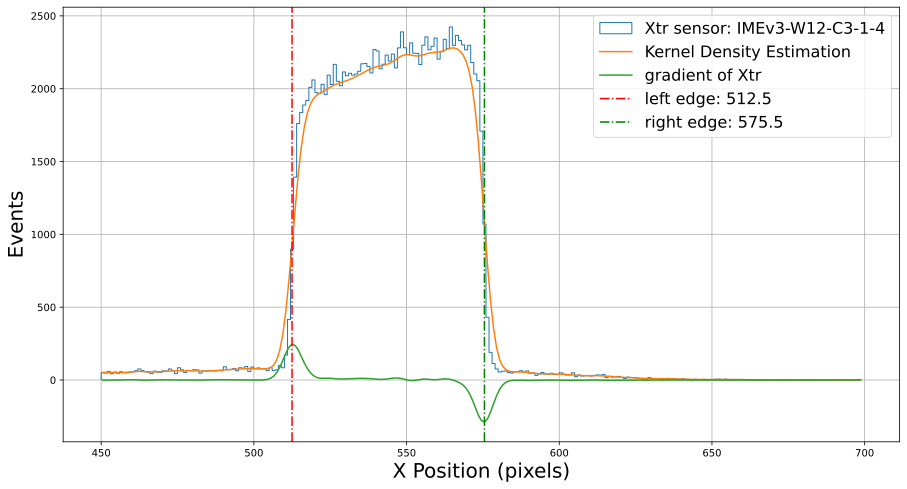
\includegraphics[width=.7\linewidth]{Images/methods/locating_edges_Xtr_batch_401_S1_DUT3.png}
    \captionsetup{width=\captionwidth}
    \caption{Projection of hits on the X axis after the \nameref{subsec:pulseHeight_cut}. By taking its derivative, it was possible to determine the position of the edges of the sensor. The unit is pixels of MIMOSA planes.}
    \label{fig:edges_of_the_sensor}
\end{figure}

Looking at the projections of hits on the X and Y coordinates, it was possible to determine the outline of the pad. The distribution was smoothed\footnote{Using a Kernel Density Estimator, as done previously for the pulse height distribution.} and its gradient (derivative) was calculated. This gave rise to two remarkably pronounced peaks shown in Figure~\ref{fig:edges_of_the_sensor}, which could be interpreted as the edges of the pads. By applying this procedure to both the X and Y projections we determined the horizontal and vertical edges, respectively. The final rectangular shape can be seen in Figure~\ref{fig:pulseHeight_cut_highlight}, alongside with the density of hits after applying a \textit{pulse height cut}. In few cases the sensors were slightly tilted in the XY plane, giving rise to slightly imprecise outlines, this is shown in \ref{fig:tilted_sensors}, although it did not have a significant impact on the rest of the analysis.

% NOTE: the edges defined like this are smaller than the real size of the pad (which is 1.3x1.3 mm\(^2\)) \cite{Agapopoulou_2022} \marginpar{\flushleft There is an outer guard ring isolating, so maybe the size is correct}

For certain properties that were analyzed (such as efficiency and time resolution) it became clear that the rough selection of the contour of the pad was not always sufficient. Thus, an additional \textit{central area cut} was set up. A region of \(0.5\times0.5\unit{\milli\meter^2}\) in the center of the pad was selected (similarly to what had been done in \cite{Agapopoulou_2022}) in order to avoid undesirable effects originating from the region outside the gain layer of the LGAD.

\begin{figure}[h!tbp]
    \centering
    \subfloat[The heatmap of the reconstructed tracks without any cuts applied. The large rectangular shape is produced by the region of interest (ROI) selected with the FE-I4.]{
        \includegraphics[width=.47\linewidth]{Images/methods/2D_Tracks_401 S1 (no cuts)_DUTs_3.png}
        \label{fig:hits_no_cuts}}
    \hfill
    \subfloat[The smaller rectangle corresponds to the area of the pad (highlighted in red with sides lengths) found by applying a \textit{pulse height cut}.]{
        \includegraphics[width=.47\linewidth]{Images/methods/2D_Tracks_401_S1 highlight geometry cut (using pulseHeight).png}
        \label{fig:pulseHeight_cut_highlight}}
    \captionsetup{width=\captionwidth}
    \caption{The events selected by applying a pulse height cut}
\end{figure}

\subsection{Time cut}\label{subsec:time_cut}

The physical distance between the MCP and the DUT was fixed, and the momentum of the particles was constant throughout all the runs. Thus, the flight time of the particles between the MCP and the DUT was peaked around one point. Using this knowledge, an additional cut on the \(\Delta t\) was applied.

Firstly, the distribution of \(\Delta t\) (\(t_{DUT}-t_{MCP}\), time of arrival of the DUT - MCP) without any other cut was fit with a Gaussian plus a uniform background (Figure~\ref{fig:time_cut_gauss+bg_fit}):

\begin{figure}[h!tbp]
    \centering
    \includegraphics[width=.9\linewidth]{Images/methods/time_difference_603_S2_gauss_fit_no_cuts_DUT2.png}
    \captionsetup{width=\captionwidth}
    \caption{Time difference distribution (\(t_{DUT}-t_{MCP}\)) fit with a Gaussian + uniform background. The vertical dashed lines represent the boundary set as \textit{time cut}. The presence of the secondary peak is explained in Section~\ref{sec:multiple_peaks}.}
    \label{fig:time_cut_gauss+bg_fit}
\end{figure}

\begin{equation*}
    f(x,A,\mu,\sigma,BG) = A \cdot e^{-\frac{1}{2}\left(\frac{x-\mu}{\sigma} \right)^2} + BG  \, .
\end{equation*}

\(A:\) Amplitude (n° of events);\quad \(\mu:\) Mean of the gaussian;\quad \(\sigma:\) Standard deviation;\quad \(BG:\) Uniform BackGround.

Ultimately, a \textit{time cut} was defined as all the events lying inside an interval of a number \(n\) of standard deviations \(\sigma\):

\begin{equation}
    (\mu-n\sigma;\mu+n\sigma) \, .
\end{equation}

Given that roughly 99.7\% of all values of a normal distribution lie within 3 standard deviations, \(n=3\) was deemed an adequate choice.

This cut proved to be especially useful in calculating the total efficiency of each pad and in fitting the charge distribution.

Although, some peculiarities became apparent, namely the second peak shifted to the right of the main one (meaning delayed compared to the latter) and some discrepancy with the expected Gaussian distribution around the left tail. These effects were further investigated and will be explained later in Sections \ref{sec:multiple_peaks} and \ref{sec:deviations_from_gaussian}.

\subsubsection{Heavily radiated sensor case}\label{subsec:geometry_cut_w/pulse_cut}

In some cases, typically for heavily radiated sensors, the noise in the pulse height distribution was too large (Figure~\ref{fig:pulseHeight_cut_failed}) to allow a \textit{pulse height cut} as in Section~\ref{subsec:pulseHeight_cut}. This happened due to the pulse height decreasing and the noise peaks rising, so the separation between the two became less marked. In these situations it was possible to apply a \textit{time cut} instead and still get a satisfactory contour of the pad. The results of the two methods were very similar (Figure~\ref{fig:geometry_cut_comparison} in \nameref{chap:appendix}) so this seemed a good alternative.

\begin{figure}[h!tbp]
    \centering
    \subfloat[Pulse height distribution, without a clear boundary between noise and signal. The orange belt represents the poissonian error.]{
        \includegraphics[width=.4\linewidth]{Images/methods/2D_Sensors_603 S2 pulseHeight cut_only_pulse.png}
        \label{fig:pulseHeight_cut_failed}}
    \hfill
    \centering
    \subfloat[Contour of the pad, highlighted in red, found by applying a time cut to the data. The irregular shape of the pad is caused by the ROI selected by the FEi4.]{
        \includegraphics[width=.55\linewidth]{Images/methods/2D_Tracks_603_S2 highlight geometry cut (using time).png}
        \label{fig:time_cut_highlight}}
    \captionsetup{width=\captionwidth}
    \caption{Example of a different sensor (irradiated), for which the previous \textit{pulse height cut} became impractical (left), but using \textit{time cut} yielded a reasonable outline of the pad (right)}
\end{figure}

\subsection{Quality cuts validation}

To qualitatively confirm the soundness of the cuts performed, we plotted the density distribution of events of \(\boldsymbol{\Delta t}\) vs \textbf{pulse height} (Figures~\ref{fig:time_pulseHeight_nocut} and \ref{fig:time_pulseHeight_center}). The left plot shows all the available tracks, the right plot shows only the tracks that pass through the smaller central area of the DUT (a square of \(0.5\times0.5\unit{\milli\meter^2}\) explained in Section~\ref{sec:geometry_cut}).

The narrow selection of events in the right plot is very likely to be real signals (as they are particles guaranteed to have passed through the sensor). By comparing it with the plot on the left it can be noticed that a horizontal cut (\nameref{subsec:pulseHeight_cut}) and two vertical cuts (\nameref{subsec:time_cut}) provide indeed a good filter for physically meaningful events. 


\begin{figure}[h!tbp]
    \centering
    \subfloat[Density plot of all the events without any cuts applied.]{
        \includegraphics[width=.47\linewidth]{Images/methods/Time_pulseHeight_401S1_DUTs_3_(3,).png}
        \label{fig:time_pulseHeight_nocut}}
    \hfill
    \centering
    \subfloat[Density plot selecting only tracks passing through the central \(0.5\times0.5\unit{\milli\meter^2}\) area of the pad.]{
        \includegraphics[width=.47\linewidth]{Images/methods/Time_pulseHeight_401S1 central area_DUTs_3_(3,).png}
        \label{fig:time_pulseHeight_center}}
    \captionsetup{width=\captionwidth}
        \caption{Density plot of events when no cuts are applied (left) and when only a central square in the sensor is selected (right). The comparison between the two plots validated our choices made for quality cuts.}
\end{figure}


\section{Collected charge}\label{sec:methods_collected_charge}

A central goal of this study was to measure the distribution of the charge collected by the pads and verify their correspondence with the theoretical distribution: a convolution of a Gaussian and a Landau distribution (Appendix \ref{sec:vavilov_vs_landau_distribution}).

To achieve this, all the quality cuts defined in Section~\ref{sec:qualtiy_cuts} were applied, and a fit was carried out using an implementation of the Gaussian*Landau convolution provided by the ROOT framework~\cite{Brun:1997pa} (Figure~\ref{fig:charge_ROOT_fit}).

The collected charge of a sensor is defined as the most probable value (MPV) of the charge, i.e. the highest point in the distribution.

\begin{figure}[h!tbp]
    \centering
    \includegraphics[width=1\linewidth]{Images/methods/charge_data_all_cuts_401_S1_3_Charge_fit_ROOT_double_plot.png}
    \captionsetup{width=\captionwidth}
    \caption{Fit of the charge distribution (red) carried out with ROOT. On the right it is shown the same plot in logarithmic scale, to highlight the extra noise at \(\approx 0\).}
    \label{fig:charge_ROOT_fit}
\end{figure}

\subsubsection{Gain}
% charged particle in 50 um of silicon produce ~0.52 fC of charge or 3280 e-h pairs
The gain is obtained by dividing the most probable value of the collected charge by the expected charge from a minimum ionizing particle (MIP) in a silicon sensor without gain. For a \qty{50}{\micro\meter} thick sensor, this value is \(3280\) e-h pairs, equivalent to \qty{.52}{\femto\coulomb} \cite{meroli_energy_loss2011}.

\subsubsection{Extra noise}
Despite all the trimming to the data, a noticeable part of the noise centered at \(\approx 0\) could not be removed. We could not pinpoint the origin of this extra noise, but a lot of factors could contribute to it: track reconstruction, other electronic noise etc.
Considering this point, the fit was performed in a smaller interval, avoiding the noise (Figure~\ref{fig:charge_ROOT_fit}). The left limit was fixed at \(4\si{fC}\), as this is also the lowest signal that the electronic board is able to measure, the right limit was adjusted to include only bins with significant amount of data (and account for the \nameref{subsec:charge_irregularities}, described in Appendix).

%%% maybe I can put a table to show which cuts I applied to which variables


\section{Efficiency}\label{sec:methods_efficiency}

The efficiency (\(\epsilon\)) was defined as the total number of tracks with charge larger than a certain \textit{threshold charge} divided by the total number of reconstructed track (\textbf{after} quality cuts had been applied).

% \begin{equation*}
%     \text{Efficiency} = \frac{\text{Tracks with } q>Q_{threshold}}{\text{Total tracks}}  \, .
% \end{equation*}

\begin{equation*}
    \epsilon = \frac{\text{Tracks with } q>Q_{threshold}}{\text{Total tracks}}  \, .
\end{equation*}

The threshold charge \(Q_{threshold}\) was chosen to be \(4\si{fC}\), which corresponds to the limit of sensitivity of the ASIC.

Before measuring the overall efficiency of the sensors, we applied a \textit{time cut} (as described in \nameref{subsec:time_cut}). Additionally, we elected to restrict the calculation to the smaller \textit{central area} of \(0.5\times0.5\unit{\milli\meter^2}\) defined earlier in Section~\ref{sec:geometry_cut}. This area can be seen highlighted in red in Figure~\ref{fig:efficiency_2D_plot}, which also shows the efficiency value computed for each individual squared binning of the surface.

Finally, the total efficiency was also computed with different values of \textit{threshold charge} to obtain the plot in Figure~\ref{fig:efficiency_depending_threshold}, which shows that (in this example) the value remains constant well after the chosen threshold of \(4\si{fC}\).

\begin{figure}[h!tbp]
    \centering
    \includegraphics[width=0.7\linewidth]{Images/methods/efficiency_plots/2D Efficiency_401_S1_with_time_cut_with_center_highlight_DUTs_3.png}
    \captionsetup{width=\captionwidth}
    \caption{2D histogram plot of the efficiency (per squared bin) and the \textit{central area cut} highlighted in red.}
    \label{fig:efficiency_2D_plot}
\end{figure}

\begin{figure}[h!tbp]
    \centering
    \includegraphics[width=0.5\linewidth]{Images/methods/efficiency_plots/Efficiency depending on threshold charge (with cuts) batch 401 S1.png}
    \captionsetup{width=\captionwidth}
    \caption{Total efficiency when changing the threshold value, ensuring that there is a large plateau of high efficiency.}
    \label{fig:efficiency_depending_threshold}
\end{figure}


\section{Time Resolution}\label{sec:methods_time_resolution}

The difference of times of arrival between the DUT and the MCP was fitted with a normal distribution. The standard deviation of said distribution corresponded to the time resolution of the DUT and MCP combined. Using simple error propagation, the time resolution of the DUT was computed: 

\begin{equation*}
    \begin{gathered}
    \sigma_{dut+MCP} = \sigma_{dut} \oplus \sigma_{MCP} \\
    \downarrow \\
    \sigma_{dut+MCP}^2 = \sigma_{dut}^2 + \sigma_{MCP}^2 \\
    \sigma_{dut} = \sqrt{\sigma_{dut+MCP}^2-\sigma_{MCP}^2}  \, .
    \end{gathered}
\end{equation*}


\begin{figure}[h!tbp]
    \centering
    \includegraphics[width=0.7\linewidth]{Images/methods/time_resolution_plots/time_difference_401_S1_zoomed_and_gauss_fit_with_cuts_central_area_DUTs_3.png}
    \captionsetup{width=\captionwidth}
    \caption{Gaussian fit of \(\Delta t\) to find the time resolution (\(\sigma\)), the error bars are the statistical poissonian error (\(y_{err}=\sqrt{N}\)). For this sensor the final time resolution was \(\sigma_{dut} = 47.72\pm0.88\si{\ps} \).}
    \label{fig:time_resolution_plot}
\end{figure}




\chapter{Results}
\marginpar{file to be created}

\chapter{Conclusions}
\marginpar{file to make}

\appendix

%%% APPENDIX
\chapter{Appendix}\label{chap:appendix}


\section[Vavilov vs Landau distribution]{On the Vavilov distribution approximation}\label{sec:vavilov_vs_landau_distribution}

% \cite[189]{NAP20066}
%     
% \maketitle
    
\begin{tcolorbox}[breakable, size=fbox, boxrule=1pt, pad at break*=1mm,colback=cellbackground, colframe=cellborder]
\prompt{In}{incolor}{1}{\boxspacing}
\begin{Verbatim}[commandchars=\\\{\}]
\PY{k+kn}{import} \PY{n+nn}{numpy} \PY{k}{as} \PY{n+nn}{np} \PY{c+c1}{\PYZsh{} NumPy}
\PY{k+kn}{from} \PY{n+nn}{scipy}\PY{n+nn}{.}\PY{n+nn}{optimize} \PY{k+kn}{import} \PY{n}{fsolve} 
\PY{k+kn}{from} \PY{n+nn}{IPython}\PY{n+nn}{.}\PY{n+nn}{display} \PY{k+kn}{import} \PY{n}{Image}
\PY{k+kn}{import} \PY{n+nn}{pandas} \PY{k}{as} \PY{n+nn}{pd} \PY{c+c1}{\PYZsh{} Pandas}
\PY{n}{pd}\PY{o}{.}\PY{n}{options}\PY{o}{.}\PY{n}{display}\PY{o}{.}\PY{n}{float\PYZus{}format} \PY{o}{=} \PY{l+s+s1}{\PYZsq{}}\PY{l+s+si}{\PYZob{}:5,.4E\PYZcb{}}\PY{l+s+s1}{\PYZsq{}}\PY{o}{.}\PY{n}{format}
\end{Verbatim}
\end{tcolorbox}

    \hypertarget{calculating-the-factor-the-determines-if-the-vavilov-distribution-can-be-approximated-by-a-landau}{%
\section{Calculating the factor the determines if the Vavilov
distribution can be approximated by a
Landau}\label{calculating-the-factor-the-determines-if-the-vavilov-distribution-can-be-approximated-by-a-landau}}

Bethe-Bloch mean energy loss: \[
\left\langle-\frac{dE}{dx} \right\rangle \frac{1}{\rho} =  K z_0^2 \frac{1}{\beta^2} \frac{Z}{A M_u} \cdot\left[\frac{1}{2}\ln \left(\frac{2m_e c^2 \beta^2 W_{max}}{I^2 \cdot (1-\beta^2)}\right) - \beta^2\right]
\]

\[
K/M_u = 4 \pi N_A r_e^2 m_e c^2 /M_u = 0.307075\space \text{MeV g}^{-1} \text{cm}^2
\]

\[
r_e  = \frac{e^2}{4\pi\varepsilon_0 m_e c^2} \\
M_u = 1 \frac{g}{mol} \quad z_0=1 \\
\left( W_{max} \equiv \epsilon_{max} \right)
\]

For \textbf{silicon}: \[
Z = 14 \\
A = 28.085 \\ 
\rho = 2.329085 \text{  g cm}^{-3}\\
I = 173 \text{ eV} % \quad \text{(mean excitation energy)}
\]

\hypertarget{calculating-beta-for-a-proton-of-energy-e_k}{%
\subsubsection{\texorpdfstring{Calculating \(\beta\) for a proton of
energy
\(E_k\)}{Calculating \textbackslash beta for a proton of energy E\_k}}\label{calculating-beta-for-a-proton-of-energy-e_k}}

\[
E_k = (\gamma - 1) m_o c^2 \\
\gamma = \frac{E_k + m_o c^2}{m_o c^2} \\
\beta^2 = 1 - \left(\frac{m_o c^2}{E_k +m_o c^2} \right)^2
\]

for a proton of energy \(E_k=120\space \text{GeV}\),
\(m_0 = 938.272\space \text{MeV/c}^2\)

    \begin{tcolorbox}[breakable, size=fbox, boxrule=1pt, pad at break*=1mm,colback=cellbackground, colframe=cellborder]
\prompt{In}{incolor}{2}{\boxspacing}
\begin{Verbatim}[commandchars=\\\{\}]
\PY{n}{energy} \PY{o}{=} \PY{l+m+mf}{120e3} \PY{c+c1}{\PYZsh{} MeV  (120 GeV)}
\PY{c+c1}{\PYZsh{} m\PYZus{}particle = 938.272088 \PYZsh{} MeV/c\PYZca{}2  protons }
\PY{n}{m\PYZus{}particle} \PY{o}{=} \PY{l+m+mf}{938.213} \PY{c+c1}{\PYZsh{} MeV/c\PYZca{}2     protons (older value)}

\PY{n}{gamma} \PY{o}{=} \PY{p}{(}\PY{n}{energy} \PY{o}{+} \PY{n}{m\PYZus{}particle}\PY{p}{)}\PY{o}{/}\PY{n}{m\PYZus{}particle}
\PY{n}{beta\PYZus{}2} \PY{o}{=} \PY{l+m+mi}{1} \PY{o}{\PYZhy{}} \PY{n}{m\PYZus{}particle}\PY{o}{*}\PY{o}{*}\PY{l+m+mi}{2}\PY{o}{/}\PY{p}{(}\PY{n}{m\PYZus{}particle} \PY{o}{+} \PY{n}{energy}\PY{p}{)}\PY{o}{*}\PY{o}{*}\PY{l+m+mi}{2}

\PY{n+nb}{print}\PY{p}{(}\PY{l+s+s2}{\PYZdq{}}\PY{l+s+s2}{ gamma: }\PY{l+s+s2}{\PYZdq{}}\PY{p}{,} \PY{n}{gamma}\PY{p}{,} \PY{l+s+s2}{\PYZdq{}}\PY{l+s+se}{\PYZbs{}n}\PY{l+s+s2}{\PYZdq{}}\PY{p}{,} \PY{l+s+s2}{\PYZdq{}}\PY{l+s+s2}{beta²: }\PY{l+s+s2}{\PYZdq{}}\PY{p}{,} \PY{n}{beta\PYZus{}2}\PY{p}{)}
\end{Verbatim}
\end{tcolorbox}

    \begin{Verbatim}[commandchars=\\\{\}]
 gamma:  128.90272571367058
 beta²:  0.999939816727599
    \end{Verbatim}

    from https://academic.oup.com/book/43645/chapter/365027598\#404941541 :

The parameter \(\kappa\) of the Vavilov distribution determines if it
becomes close to a Landau (\(\kappa\rightarrow0\)) or a Gaussian
(\(\kappa 10\)).

To calculate \(\kappa\): 
\[
\kappa = \frac{\xi}{\epsilon_{max}}
\]

where: \[
\xi = \frac{1}{2} K \frac{Z}{A} \frac{s} {\beta^2}
\]

\(s = \Delta x \cdot \rho\)

and from https://nap.nationalacademies.org/read/20066/chapter/10\#188 :
\[
\epsilon_{max} = \frac{2m_e c^2 \beta^2}{1-\beta^2}\left[ 1 + \frac{2m_e}{M}\frac{1}{\sqrt{1-\beta^2}} + \left(\frac{m_e}{M}\right)^2 \right]^{-1}
\]

where \(M\) is the mass of the incoming particle.

Also written as:

\[
\epsilon_{max} = \frac{2m_e c^2 \beta^2 \gamma^2} { 1 + \frac{2\gamma m_e}{M} + \left(\frac{m_e}{M}\right)^2}
\]

    \hypertarget{applying-this-to-a-thin-silicon-layer-50mu-textm}{%
\subsubsection{\texorpdfstring{Applying this to a thin silicon layer
(50\(\mu \text{m}\))}{Applying this to a thin silicon layer (50\textbackslash mu \textbackslash text\{m\})}}\label{applying-this-to-a-thin-silicon-layer-50mu-textm}}

(The masses are either multiplied by \(c^2\) or in a ratio, the mass
units used are \(\text{MeV}/c^2\))

    \begin{tcolorbox}[breakable, size=fbox, boxrule=1pt, pad at break*=1mm,colback=cellbackground, colframe=cellborder]
\prompt{In}{incolor}{3}{\boxspacing}
\begin{Verbatim}[commandchars=\\\{\}]
\PY{c+c1}{\PYZsh{}\PYZsh{}\PYZsh{} variables values}
\PY{n}{m\PYZus{}electron} \PY{o}{=} \PY{l+m+mf}{0.51099895} \PY{c+c1}{\PYZsh{} MeV/c\PYZca{}2}
\PY{n}{z\PYZus{}0} \PY{o}{=} \PY{l+m+mi}{1} \PY{c+c1}{\PYZsh{} electric charge of incoming particle}
\PY{n}{delta\PYZus{}x} \PY{o}{=} \PY{l+m+mf}{5e\PYZhy{}3} \PY{c+c1}{\PYZsh{} cm  (50um)}

\PY{c+c1}{\PYZsh{}\PYZsh{}\PYZsh{} silicon}
\PY{n}{Z} \PY{o}{=} \PY{l+m+mi}{14}   \PY{c+c1}{\PYZsh{} atomic number}
\PY{n}{A} \PY{o}{=} \PY{l+m+mf}{28.085}  \PY{c+c1}{\PYZsh{} atomic weight}
\PY{n}{density} \PY{o}{=} \PY{l+m+mf}{2.329085} \PY{c+c1}{\PYZsh{} g cm\PYZca{}\PYZhy{}3}
\PY{n}{mean\PYZus{}excitation} \PY{o}{=} \PY{l+m+mf}{173e\PYZhy{}6} \PY{c+c1}{\PYZsh{} MeV  (mean excitation energy of Silicon: 173 eV)}

\PY{n}{s} \PY{o}{=} \PY{n}{delta\PYZus{}x} \PY{o}{*} \PY{n}{density} \PY{c+c1}{\PYZsh{} g cm\PYZca{}\PYZhy{}2}
\PY{n}{K} \PY{o}{=} \PY{l+m+mf}{0.307075} \PY{c+c1}{\PYZsh{} MeV g\PYZca{}\PYZhy{}1 cm\PYZca{}2}
\end{Verbatim}
\end{tcolorbox}

    \begin{tcolorbox}[breakable, size=fbox, boxrule=1pt, pad at break*=1mm,colback=cellbackground, colframe=cellborder]
\prompt{In}{incolor}{4}{\boxspacing}
\begin{Verbatim}[commandchars=\\\{\}]
\PY{k}{def} \PY{n+nf}{xi\PYZus{}func}\PY{p}{(}\PY{n}{energy}\PY{p}{)}\PY{p}{:}
    \PY{n}{beta\PYZus{}2} \PY{o}{=} \PY{l+m+mi}{1} \PY{o}{\PYZhy{}} \PY{n}{m\PYZus{}particle}\PY{o}{*}\PY{o}{*}\PY{l+m+mi}{2}\PY{o}{/}\PY{p}{(}\PY{n}{m\PYZus{}particle} \PY{o}{+} \PY{n}{energy}\PY{p}{)}\PY{o}{*}\PY{o}{*}\PY{l+m+mi}{2}
    \PY{k}{return} \PY{p}{(}\PY{l+m+mi}{1}\PY{o}{/}\PY{l+m+mi}{2} \PY{o}{*} \PY{n}{K}\PY{p}{)} \PY{o}{*} \PY{p}{(}\PY{n}{Z} \PY{o}{/} \PY{n}{A}\PY{p}{)} \PY{o}{*} \PY{p}{(}\PY{n}{s} \PY{o}{/} \PY{n}{beta\PYZus{}2}\PY{p}{)}

\PY{k}{def} \PY{n+nf}{eps\PYZus{}max\PYZus{}func}\PY{p}{(}\PY{n}{energy}\PY{p}{)}\PY{p}{:}
    \PY{n}{gamma} \PY{o}{=} \PY{p}{(}\PY{n}{energy} \PY{o}{+} \PY{n}{m\PYZus{}particle}\PY{p}{)}\PY{o}{/}\PY{n}{m\PYZus{}particle}
    \PY{n}{beta\PYZus{}2} \PY{o}{=} \PY{l+m+mi}{1} \PY{o}{\PYZhy{}} \PY{n}{m\PYZus{}particle}\PY{o}{*}\PY{o}{*}\PY{l+m+mi}{2}\PY{o}{/}\PY{p}{(}\PY{n}{m\PYZus{}particle} \PY{o}{+} \PY{n}{energy}\PY{p}{)}\PY{o}{*}\PY{o}{*}\PY{l+m+mi}{2}
    \PY{k}{return} \PY{p}{(}\PY{l+m+mi}{2} \PY{o}{*} \PY{n}{m\PYZus{}electron} \PY{o}{*} \PY{n}{beta\PYZus{}2} \PY{o}{*} \PY{n}{gamma}\PY{o}{*}\PY{o}{*}\PY{l+m+mi}{2}\PY{p}{)} \PY{o}{/} \PY{p}{(}\PY{l+m+mi}{1} \PY{o}{+} \PY{l+m+mi}{2}\PY{o}{*}\PY{n}{gamma}\PY{o}{*}\PY{n}{m\PYZus{}electron}\PY{o}{/}\PY{n}{m\PYZus{}particle} \PY{o}{+} \PY{p}{(}\PY{n}{m\PYZus{}electron}\PY{o}{/}\PY{n}{m\PYZus{}particle}\PY{p}{)}\PY{o}{*}\PY{o}{*}\PY{l+m+mi}{2}\PY{p}{)} \PY{c+c1}{\PYZsh{} MeV}

\PY{k}{def} \PY{n+nf}{kappa\PYZus{}func}\PY{p}{(}\PY{n}{energy}\PY{p}{,} \PY{n}{kappa\PYZus{}value}\PY{o}{=}\PY{l+m+mf}{0.01}\PY{p}{)}\PY{p}{:}
    \PY{l+s+sd}{\PYZdq{}\PYZdq{}\PYZdq{}kappa as a function of the energy (to find the zeros for k=kappa\PYZus{}value)\PYZdq{}\PYZdq{}\PYZdq{}}
    \PY{n}{gamma} \PY{o}{=} \PY{p}{(}\PY{n}{energy} \PY{o}{+} \PY{n}{m\PYZus{}particle}\PY{p}{)}\PY{o}{/}\PY{n}{m\PYZus{}particle}
    \PY{n}{beta\PYZus{}2} \PY{o}{=} \PY{l+m+mi}{1} \PY{o}{\PYZhy{}} \PY{n}{m\PYZus{}particle}\PY{o}{*}\PY{o}{*}\PY{l+m+mi}{2}\PY{o}{/}\PY{p}{(}\PY{n}{m\PYZus{}particle} \PY{o}{+} \PY{n}{energy}\PY{p}{)}\PY{o}{*}\PY{o}{*}\PY{l+m+mi}{2}
    \PY{k}{return} \PY{n}{xi\PYZus{}func}\PY{p}{(}\PY{n}{energy}\PY{p}{)} \PY{o}{/} \PY{n}{eps\PYZus{}max\PYZus{}func}\PY{p}{(}\PY{n}{energy}\PY{p}{)} \PY{o}{\PYZhy{}} \PY{n}{kappa\PYZus{}value}
\end{Verbatim}
\end{tcolorbox}

    \begin{tcolorbox}[breakable, size=fbox, boxrule=1pt, pad at break*=1mm,colback=cellbackground, colframe=cellborder]
\prompt{In}{incolor}{5}{\boxspacing}
\begin{Verbatim}[commandchars=\\\{\}]
\PY{n}{xi} \PY{o}{=} \PY{p}{(}\PY{l+m+mi}{1}\PY{o}{/}\PY{l+m+mi}{2} \PY{o}{*} \PY{n}{K}\PY{p}{)} \PY{o}{*} \PY{p}{(}\PY{n}{Z} \PY{o}{/} \PY{n}{A}\PY{p}{)} \PY{o}{*} \PY{p}{(}\PY{n}{s} \PY{o}{/} \PY{n}{beta\PYZus{}2}\PY{p}{)} \PY{c+c1}{\PYZsh{} MeV}

\PY{n}{epsilon\PYZus{}max} \PY{o}{=} \PY{n}{eps\PYZus{}max\PYZus{}func}\PY{p}{(}\PY{n}{energy}\PY{p}{)} \PY{c+c1}{\PYZsh{} MeV}

\PY{n}{kappa} \PY{o}{=} \PY{n}{xi} \PY{o}{/} \PY{n}{epsilon\PYZus{}max}

\PY{n+nb}{print}\PY{p}{(}\PY{l+s+s2}{\PYZdq{}}\PY{l+s+s2}{k =}\PY{l+s+s2}{\PYZdq{}}\PY{p}{,}\PY{n}{kappa}\PY{p}{)}
\end{Verbatim}
\end{tcolorbox}

    \begin{Verbatim}[commandchars=\\\{\}]
k = 5.98637846070628e-08
    \end{Verbatim}

    \hypertarget{comparison-with-calculations-from-httpsnap.nationalacademies.orgread20066chapter10189}{%
\subsection{Comparison with calculations from \cite{NAP20066} }\label{comparison-with-calculations-from-httpsnap.nationalacademies.orgread20066chapter10189}}

    \begin{tcolorbox}[breakable, size=fbox, boxrule=1pt, pad at break*=1mm,colback=cellbackground, colframe=cellborder]
\prompt{In}{incolor}{6}{\boxspacing}
\begin{Verbatim}[commandchars=\\\{\}]
\PY{n}{Image}\PY{p}{(}\PY{l+s+s2}{\PYZdq{}}\PY{l+s+s2}{epsilon and xi formulas.png}\PY{l+s+s2}{\PYZdq{}}\PY{p}{,} \PY{n}{width}\PY{o}{=}\PY{l+m+mi}{1000}\PY{p}{)}
\end{Verbatim}
\end{tcolorbox}
 
            
\prompt{Out}{outcolor}{6}{}
    
    \begin{center}
    \adjustimage{max size={0.9\linewidth}{0.9\paperheight}}{Chapters/Vavilov_Landau/output_10_0.png}
    \end{center}
    { \hspace*{\fill} \\}
    

    Then follows a table with the values calculated for different energies:

    \begin{tcolorbox}[breakable, size=fbox, boxrule=1pt, pad at break*=1mm,colback=cellbackground, colframe=cellborder]
\prompt{In}{incolor}{7}{\boxspacing}
\begin{Verbatim}[commandchars=\\\{\}]
\PY{n}{Image}\PY{p}{(}\PY{l+s+s2}{\PYZdq{}}\PY{l+s+s2}{Table of k and xi values.png}\PY{l+s+s2}{\PYZdq{}}\PY{p}{,} \PY{n}{width}\PY{o}{=}\PY{l+m+mi}{800}\PY{p}{)}
\end{Verbatim}
\end{tcolorbox}
 
            
\prompt{Out}{outcolor}{7}{}
    
    \begin{center}
    \adjustimage{max size={0.9\linewidth}{0.9\paperheight}}{Chapters/Vavilov_Landau/output_12_0.png}
    \end{center}
    { \hspace*{\fill} \\}
    

    Comparison of these values with my previous calculations

    \begin{tcolorbox}[breakable, size=fbox, boxrule=1pt, pad at break*=1mm,colback=cellbackground, colframe=cellborder]
\prompt{In}{incolor}{8}{\boxspacing}
\begin{Verbatim}[commandchars=\\\{\}]
\PY{c+c1}{\PYZsh{} Values from 100 MeV to 10 GeV}
\PY{n}{energy\PYZus{}array} \PY{o}{=} \PY{n}{np}\PY{o}{.}\PY{n}{array}\PY{p}{(}\PY{p}{[}\PY{l+m+mi}{100}\PY{p}{,}\PY{l+m+mi}{150}\PY{p}{,}\PY{l+m+mi}{200}\PY{p}{,}\PY{l+m+mi}{300}\PY{p}{,}\PY{l+m+mi}{400}\PY{p}{,}\PY{l+m+mi}{500}\PY{p}{,}\PY{l+m+mi}{600}\PY{p}{,}\PY{l+m+mi}{800}\PY{p}{,}\PY{l+m+mi}{1000}\PY{p}{,}\PY{l+m+mi}{1500}\PY{p}{,}\PY{l+m+mi}{2000}\PY{p}{,}\PY{l+m+mi}{3000}\PY{p}{,}\PY{l+m+mi}{4000}\PY{p}{,}\PY{l+m+mi}{5000}\PY{p}{,}\PY{l+m+mi}{6000}\PY{p}{,}\PY{l+m+mi}{8000}\PY{p}{,}\PY{l+m+mi}{10000}\PY{p}{]}\PY{p}{)}
\end{Verbatim}
\end{tcolorbox}

    \begin{tcolorbox}[breakable, size=fbox, boxrule=1pt, pad at break*=1mm,colback=cellbackground, colframe=cellborder]
\prompt{In}{incolor}{9}{\boxspacing}
\begin{Verbatim}[commandchars=\\\{\}]
\PY{n}{table\PYZus{}data} \PY{o}{=} \PY{n}{np}\PY{o}{.}\PY{n}{vstack}\PY{p}{(}\PY{p}{(}\PY{l+m+mi}{1} \PY{o}{\PYZhy{}} \PY{n}{m\PYZus{}particle}\PY{o}{*}\PY{o}{*}\PY{l+m+mi}{2} \PY{o}{/} \PY{p}{(}\PY{n}{m\PYZus{}particle}\PY{o}{+}\PY{n}{energy\PYZus{}array}\PY{p}{)}\PY{o}{*}\PY{o}{*}\PY{l+m+mi}{2}\PY{p}{,}
              \PY{n}{eps\PYZus{}max\PYZus{}func}\PY{p}{(}\PY{n}{energy\PYZus{}array}\PY{p}{)}\PY{p}{,}
              \PY{n}{A}\PY{o}{/}\PY{n}{Z} \PY{o}{*} \PY{n}{xi\PYZus{}func}\PY{p}{(}\PY{n}{energy\PYZus{}array}\PY{p}{)} \PY{o}{/} \PY{n}{s}\PY{p}{,}
              \PY{n}{A}\PY{o}{/}\PY{n}{Z} \PY{o}{*} \PY{n}{kappa\PYZus{}func}\PY{p}{(}\PY{n}{energy\PYZus{}array}\PY{p}{,}\PY{n}{kappa\PYZus{}value}\PY{o}{=}\PY{l+m+mi}{0}\PY{p}{)} \PY{o}{/} \PY{n}{s}\PY{p}{)}\PY{p}{)}

\PY{n}{df} \PY{o}{=} \PY{n}{pd}\PY{o}{.}\PY{n}{DataFrame}\PY{p}{(}\PY{n}{data}\PY{o}{=}\PY{n}{table\PYZus{}data}\PY{o}{.}\PY{n}{transpose}\PY{p}{(}\PY{p}{)}\PY{p}{,} \PY{n}{columns}\PY{o}{=}\PY{p}{(}\PY{l+s+s2}{\PYZdq{}}\PY{l+s+s2}{\PYZdl{}}\PY{l+s+se}{\PYZbs{}\PYZbs{}}\PY{l+s+s2}{beta \PYZca{}2\PYZdl{}}\PY{l+s+s2}{\PYZdq{}}\PY{p}{,}\PY{l+s+s2}{\PYZdq{}}\PY{l+s+s2}{\PYZdl{}}\PY{l+s+s2}{\PYZbs{}}\PY{l+s+s2}{epsilon\PYZus{}}\PY{l+s+si}{\PYZob{}max\PYZcb{}}\PY{l+s+s2}{\PYZdl{}}\PY{l+s+s2}{\PYZdq{}}\PY{p}{,}\PY{l+s+s2}{\PYZdq{}}\PY{l+s+s2}{\PYZdl{}A/Z*}\PY{l+s+se}{\PYZbs{}\PYZbs{}}\PY{l+s+s2}{xi/s\PYZdl{}}\PY{l+s+s2}{\PYZdq{}}\PY{p}{,}\PY{l+s+s2}{\PYZdq{}}\PY{l+s+s2}{\PYZdl{}A/Z*}\PY{l+s+s2}{\PYZbs{}}\PY{l+s+s2}{kappa/s\PYZdl{}}\PY{l+s+s2}{\PYZdq{}}\PY{p}{)}\PY{p}{)}
\PY{n}{df}\PY{o}{.}\PY{n}{insert}\PY{p}{(}\PY{l+m+mi}{0}\PY{p}{,} \PY{l+s+s2}{\PYZdq{}}\PY{l+s+s2}{Energy}\PY{l+s+s2}{\PYZdq{}}\PY{p}{,} \PY{n}{pd}\PY{o}{.}\PY{n}{DataFrame}\PY{p}{(}\PY{n}{energy\PYZus{}array}\PY{p}{,}\PY{n}{dtype}\PY{o}{=}\PY{n}{np}\PY{o}{.}\PY{n}{int\PYZus{}}\PY{p}{)}\PY{p}{)}

\PY{n}{display}\PY{p}{(}\PY{n}{df}\PY{p}{)}
\end{Verbatim}
\end{tcolorbox}

    
    \begin{Verbatim}[commandchars=\\\{\}]
    Energy  \$\textbackslash{}beta \^{}2\$  \$\textbackslash{}epsilon\_\{max\}\$  \$A/Z*\textbackslash{}xi/s\$  \$A/Z*\textbackslash{}kappa/s\$
0      100  1.8336E-01        2.2919E-01   8.3735E-01      3.6534E+00
1      150  2.5668E-01        3.5247E-01   5.9816E-01      1.6971E+00
2      200  3.2055E-01        4.8153E-01   4.7898E-01      9.9471E-01
3      300  4.2587E-01        7.5699E-01   3.6053E-01      4.7627E-01
4      400  5.0847E-01        1.0556E+00   3.0196E-01      2.8607E-01
5      500  5.7444E-01        1.3773E+00   2.6728E-01      1.9407E-01
6      600  6.2798E-01        1.7221E+00   2.4450E-01      1.4198E-01
7      800  7.0866E-01        2.4809E+00   2.1666E-01      8.7329E-02
8     1000  7.6569E-01        3.3321E+00   2.0052E-01      6.0178E-02
9     1500  8.5193E-01        5.8636E+00   1.8022E-01      3.0736E-02
10    2000  8.9804E-01        8.9708E+00   1.7097E-01      1.9059E-02
11    3000  9.4324E-01        1.6908E+01   1.6278E-01      9.6272E-03
12    4000  9.6390E-01        2.7135E+01   1.5929E-01      5.8701E-03
13    5000  9.7504E-01        3.9646E+01   1.5747E-01      3.9719E-03
14    6000  9.8171E-01        5.4431E+01   1.5640E-01      2.8733E-03
15    8000  9.8898E-01        9.0793E+01   1.5525E-01      1.7099E-03
16   10000  9.9264E-01        1.3616E+02   1.5468E-01      1.1360E-03
    \end{Verbatim}

    
    \hypertarget{at-what-energy-gamma-the-value-kappa-0.01}{%
\subsection{\texorpdfstring{At what energy (\(\gamma\)) the value
\(\kappa = 0.01\)}{At what energy (\textbackslash gamma) the value \textbackslash kappa = 0.01}}\label{at-what-energy-gamma-the-value-kappa-0.01}}

    \begin{tcolorbox}[breakable, size=fbox, boxrule=1pt, pad at break*=1mm,colback=cellbackground, colframe=cellborder]
\prompt{In}{incolor}{10}{\boxspacing}
\begin{Verbatim}[commandchars=\\\{\}]
\PY{n}{kappa\PYZus{}value} \PY{o}{=} \PY{l+m+mf}{0.01}

\PY{n}{target\PYZus{}energy} \PY{o}{=} \PY{n}{fsolve}\PY{p}{(}\PY{n}{kappa\PYZus{}func}\PY{p}{,} \PY{n}{x0}\PY{o}{=}\PY{l+m+mi}{500}\PY{p}{,} \PY{n}{args}\PY{o}{=}\PY{p}{(}\PY{n}{kappa\PYZus{}value}\PY{p}{)}\PY{p}{)}
\PY{n+nb}{print}\PY{p}{(}\PY{n}{target\PYZus{}energy}\PY{p}{[}\PY{l+m+mi}{0}\PY{p}{]}\PY{p}{,} \PY{l+s+s2}{\PYZdq{}}\PY{l+s+s2}{MeV}\PY{l+s+s2}{\PYZdq{}}\PY{p}{)}
\end{Verbatim}
\end{tcolorbox}

    \begin{Verbatim}[commandchars=\\\{\}]
148.80746742515953 MeV
    \end{Verbatim}


    % Add a bibliography block to the postdoc
    


%%% I need to replace the \si with \qty or \num or \unit

The theoretical distribution of the energy loss of heavy particles hitting a thin target has been solved rigorously by Vavilov in \cite{vavilov_1957}. The namesake distribution is a generalization of the Landau distribution, but its evaluation is more difficult, as it is expressed as an integral over some complicated functions \cite[Eq.(4)]{vavilov_1957}. Fortunately, it can be approximated by more straightforward distributions depending on the value of a parameter $\kappa$ (Eq. \eqref{eq:kappa_definition}): for $\kappa\rightarrow0$ the Vavilov distribution can be approximated by a Langau, for $\kappa>>1$ by a Gaussian. 
In this section we have replicated the calculations done in \cite{NAP20066} applied to our specific case to ensure that the Landau approximation is valid.

% \subsection{The \(\kappa\) factor}
\subsection{Vavilov approximation parameter} % remove $\kappa$ because of hyperref for now

The parameter \(\kappa\) is defined as:

\begin{equation}\label{eq:kappa_definition}
    \kappa = \frac{\xi}{\epsilon_{max}}
\end{equation}

where $\xi$ and $\epsilon_{max}$ \cite[Eq.(1)]{NAP20066} are:

\begin{equation*}
    \xi = \frac{1}{2} K \frac{Z}{A} \frac{s} {\beta^2}; \qquad s = \Delta x \cdot \rho
\end{equation*}

\begin{equation*}
\epsilon_{max} = \frac{2m_e c^2 \beta^2}{1-\beta^2}\left[ 1 + \frac{2m_e}{M}\frac{1}{\sqrt{1-\beta^2}} + \left(\frac{m_e}{M}\right)^2 \right]^{-1}
\end{equation*}


% \subsection[Vavilov distribution factor]{Calculating the $\kappa$ factor}\label{vavilov_distribution_factor}
The parameters just mentioned are the same that appear in the Bethe-Bloch mean energy loss:
\begin{equation*}
    \left\langle-\frac{dE}{dx} \right\rangle \frac{1}{\rho} =  K z_0^2 \frac{1}{\beta^2} \frac{Z}{A M_u} \cdot\left[\frac{1}{2}\ln \left(\frac{2m_e c^2 \beta^2 W_{max}}{I^2 \cdot (1-\beta^2)}\right) - \beta^2\right]
\end{equation*}

And they have the following values:

\begin{equation*}
    \frac{K}{M_u} = 4 \pi N_A r_e^2 m_e c^2 /M_u = 0.307075 \si{MeV.g^{-1}.cm^2}
\end{equation*}


\begin{equation*}
r_e = \frac{e^2}{4\pi\varepsilon_0 m_e c^2}; \qquad
M_u = 1 \frac{\si{g}}{\si{mol}}; \qquad z_0=1; \qquad
\left( W_{max} \equiv \epsilon_{max} \right)
\end{equation*}

For the case of \textbf{silicon}:
\begin{equation*}
    Z = 14; \qquad
    A = 28.085; \qquad
    \rho = 2.329085 \si{g.cm^{-3}}; \qquad
    I = 173 \si{eV} \footnote[1]{Mean excitation Energy}
\end{equation*}

Finally, for a Pion ($M=139.570\si{MeV/c^2}$) with energy $E=120\si{GeV}$ ($\gamma=860.78$ and $\beta^2=0.99999865$) and the thin layer ($50\si{\micro\meter}$) of an LGAD sensor, we obtained a value:

\begin{equation}\label{eq:kappa_value}
    \kappa = \num{8.5959e-09}
\end{equation}

Well within the Landau approximation.

Reversing the calculation and fixing $\kappa=0.01$, which is approximately the lower limit of validity, the energy of the particle should be below: $491.9\si{MeV}$. 





\section{Dead pixels line}

Some batches (for example Figure~\ref{fig:hits_no_cuts}) presented an empty vertical line, even before any data processing had been applied. By inspecting the data of the hits registered by each individual MIMOSA plane, it was found that one device had a dead column of pixels, which interfered with the track reconstruction. This problem turned out to be inconsequential for the analysis, except for reduced statistics in that very small region.

\begin{figure}[h!tbp]
    \centering
    \includegraphics[width=.9\linewidth]{Images/appendix/hits_MIMOSA4.png}
    \caption{The hits heatmap of the MIMOSA plane n°4, which shows clearly the dead column of pixels, the source of the "empty line" that appeared in the data.}
    \label{fig:MIMOSA4_hits}
\end{figure}


\section{Mislabeled sensor}\label{sec:mislabeled_sensor}

One specific sensor had three channels connected to the readout board (IMEv3-W12-2x2-1.5E15, i.e. an array of 2x2 pads from IME, with fluence of \qty{1.5e15}{\neutroneq}), but, when plotting the outline of each pad, one of them did not match the expected configuration. Additionally, in the logbook of the test beam of May 2023, there was some contradicting information regarding the connected channels on the readout board. We suspect that the inconsistent sensor could actually be one of the pads of IMEv3-W12-\textbf{1x3}-1.5E15 but, for an unfortunate coincidence, that sensor had no useful batches. %% (most likely cut out of the FEi4 ROI).
Therefore, it was not possible to confirm that the two channels were simply swapped, and Channel4 of the IMEv3-W12-2x2-1.5E15 was excluded from the analysis.


\begin{figure}[h!tbp]
    \centering
    \includegraphics[width=.9\linewidth]{Images/appendix/2D_Sensors_605 S1 (pulseHeight cut)_overlapping_v3.png}
    \caption{This plot combines the 2D plot of the reconstructed tracks (after a \textit{pulse height cut}) of the three channels of IMEv3-W12-2x2-1.5E15. It is very obvious that Channel4 does not match the expected shape of a 2x2 grid, and it is very likely wrongly labeled.}
    \label{fig:mislabeled_sensor}
\end{figure}

%%% TODO: more description instead of just additional plots?
%%% TODO: also add plots of tilted sensors (batch 203)
\section{Supplementary Figures}\label{sec:additional_plots}

\begin{figure}[h!tbp]
    \centering
    \subfloat[Using pulse height cut]{
        \includegraphics[width=.48\textwidth]{Images/appendix/2D_Tracks_401_S1 highlight geometry cut (using pulseHeight).png}
        \label{fig:geometry_cut_using_pulseHeight}}
    \hfill
    \centering
    \subfloat[Using time cut. Used only in the case of some irradiated sensors, when the noise was too high.]{
        \includegraphics[width=.48\textwidth]{Images/appendix/2D_Tracks_401_S1 highlight geometry cut (using time).png}
        \label{fig:geometry_cut_using_time}}
    \caption{Example of the \textit{geometry cut} (red rectangles) obtained by applying a \textit{pulse height cut} (left) and a \textit{time cut} (left) to show that they produce comparable results. In practice, since all results were calculated inside the smaller \ \(0.5\times0.5\unit{\milli\meter^2}\) area, there were no real differences.}
    \label{fig:geometry_cut_comparison}
\end{figure}


\begin{figure}[h!tbp]
    \centering
    \includegraphics[width=0.9\linewidth]{Images/appendix/CFD_comparison_401 central area cuts S1 dut: 3.png}
    \caption{Comparison of the fit for the time resolution of an unirradiated sensor (IMEv3-W12-1x3), for three different values of CFD: 20\%, 50\% and 70\%}
    \label{fig:CFD_comparison_unirradiated}
\end{figure}

\begin{figure}[h!tbp]
    \centering
    \includegraphics[width=0.9\linewidth]{Images/appendix/CFD_comparison_605 central area cuts S1 dut: 1.png}
    \caption{Comparison of the fit for the time resolution of an irradiated sensor (IMEv3-W12-2x2-1.5E15), for three different values of CFD: 20\%, 50\% and 70\%}
    \label{fig:CFD_comparison_irradiated}
\end{figure}


\begin{figure}[h!tbp]
    \centering
    \includegraphics[width=0.8\linewidth]{Images/appendix/2D_Tracks_203 S1 (w. time cut).png}
    \caption{An example of two sensors slightly tilted.}
    \label{fig:tilted_sensors}
\end{figure}


% \begin{figure}[h!tbp]
%     \centering
%     \includegraphics[width=0.7\linewidth]{Images/appendix/Charge_distribution_different_cuts_batch_401_S1_DUTs_3.png}
%     \caption{The different quality cuts applied and their individual effect on the charge distribution}
%     \label{fig:charge_plot_all_cuts}
% \end{figure}


% \begin{landscape}

% \begin{table}[h]
%     \caption{Complete list of the tested devices with additional details}
%     \label{tab:full_devices_tested}
%     \scriptsize
%         \begin{tabularx}{\textheight}{|l|l|l|l|l|l|l|l|X|}
%             \hline
%             \textbf{Device name} & \textbf{Vendor} & \textbf{Sensor ID} &  \begin{tabular}{@{}l@{}}\textbf{Pads,} \\ \textbf{used channels}\end{tabular} & \begin{tabular}{@{}l@{}}\textbf{Fluence} \\ \([n_{eq}/\si{cm^2}]\) \end{tabular} &\begin{tabular}{@{}l@{}} \textbf{Radiation} \\ \textbf{type} \end{tabular} & \textbf{Board name} & \begin{tabular}{@{}l@{}}\textbf{Board} \\ \textbf{channels} \end{tabular} & \textbf{Notes} \\
%             \hline
%             CNM-W4 & CNM & CNM-R15973-W4-D168 & single & 0 & - & JSI-B12 & - & reference \\ 
%             CNM-W5 & CNM & CNM-R15973-W5-D138 & single & 0 & - & JSI-B14 & - & reference \\ 
%             CNM-W5-1.5E15 & CNM & CNM-R15973-W5-D29 & single & \(\num{1.50E+15}\) & neutron & JSI-B5 & - & \\ 
%             CNM-W3-2.5E15 & CNM & CNM-R15973-W3-D29 & single & \(\num{2.50E+15}\) & neutron & JSI-PP1 & - & \\
%             USTC2.1-W17 & USTC & USTC2.1-W17-P6-A-2x2 & 2x2, 2 channels & 0 & - & CERN-3 & Ch1,Ch2 & \\
%             USTC2.1-W19 & USTC & USTC2.1-W19-P5-A-1x1 & single & 0 & - & CERN-3 & - & not tested \\
%             USTC2.1-W17-2E14 & USTC & USTC2.1-W17-P6-A-2x2 & 2x2, 1 channel & 0 & - & JSI-B2 & - & missing \\ 
%             IMEv3-W12-2x2 & IHEP & IMEv3-W12-C2-2-2 & 2x2, 2 channels & 0 & - & CERN-1 & Ch1,Ch2 &  \\ 
%             IMEv3-W12-1x3 & IHEP & IMEv3-W12-C3-1-4(and 5) & 1x3, 2 channels & 0 & - & CERN-1 & Ch3,Ch4 &  \\ 
%             IMEv3-W12-2x2-1.5E15 & IHEP & IMEv3-W12-B2-2-9-1 & 2x2, 3 channels & \(\num{1.50E+15}\) & neutron & CERN-2 & Ch0,Ch1,Ch2 &  \\ 
%             IMEv3-W16-1x3-1.5E15 & IHEP & IMEv3-W16-Q4-D4-1-4 & 1x3, 1 channel & \(\num{1.50E+15}\) & neutron & CERN-2 & Ch3 &  \\ 
%             IMEv2-W7-1E14 & IHEP & W7-II-C2-1-7IMEv2-W7Q2 & single & \(\num{1.00E+14}\) & proton & JSI-B6 & - &  \\ 
%             IMEv2-W7-6.5E14 & IHEP & W7-II-C2-1-7IMEv2-W7Q2 & single & \(\num{6.50E+14}\) & proton & JSI-PP4 & - &  \\ 
%             IMEv3-W16-8E14 & IHEP & IHEP-IMEv3-W16-Q4-D3-1-4 & single & \(\num{8.00E+14}\) & proton & JSI-B7 & - &  \\ 
%             IMEv3-W16-2.5E15 & IHEP & IHEP-IMEv3-W16-Q4-E3-1-4 & single & \(\num{2.50E+15}\) & neutron & JSI-B13 & - &  \\ 
%             \hline
%         \end{tabularx}
% \end{table}
% \end{landscape}

\FloatBarrier

\section{Tables of results}

Here are reported the tables containing all the results, divided by sensor. The column "Batch" indicates the batch number, the oscilloscope ('S1' or 'S2') and the channel number; multiple entries of a single batch number refer to multiple connected pads. The batch numbered \(5031\) was originally numbered \(503\), but it was divided into two batches because there was a significant shift in the position of the DUTs. \(5032\) was later removed due to the redundancy and higher noise.

%% All the tables with the results:
%%% CNM-W4
\begin{table}[htbp]
    \scriptsize
    \centering
    \caption{Summary of the results for the sensor: CNM-W4.}
    \label{tab:results_CNM-W4}
    \begin{tabular}{ccccccccccc}
\toprule
 &  &  & Temp. [°C] & Angle [°] & Volt. [V] & Charge [fC] & \(\pm\sigma\) [fC] & Time res. [ps] & \(\pm\sigma\) [ps] & Eff. \\
\midrule
409 & S2 & Ch3 & 21.7 & 0 & -175 & 23.61 & 0.03 & 27.76 & 1.37 & 0.997 \\
410 & S2 & Ch3 & 21.8 & 0 & -175 & 23.66 & 0.04 & 30.55 & 0.70 & 0.996 \\
408 & S2 & Ch3 & 21.4 & 0 & -160 & 16.20 & 0.02 & 36.41 & 1.18 & 0.996 \\
301 & S2 & Ch3 & 21.8 & 0 & -150 & 13.32 & 0.01 & 38.01 & 0.96 & 0.997 \\
407 & S2 & Ch3 & -30.0 & 0 & -120 & 24.98 & 0.02 & 26.78 & 1.21 & 0.997 \\
413 & S2 & Ch3 & -30.2 & 6 & -120 & 25.60 & 0.03 & 30.04 & 0.27 & 0.999 \\
411 & S2 & Ch3 & -29.6 & 13 & -120 & 28.94 & 0.03 & 25.71 & 1.44 & 0.999 \\
402 & S2 & Ch3 & -29.9 & 0 & -100 & 14.27 & 0.01 & 30.68 & 1.09 & 0.995 \\
414 & S2 & Ch3 & -31.9 & 6 & -100 & 15.03 & 0.01 & 41.60 & 0.31 & 0.998 \\
401 & S2 & Ch3 & -30.6 & 0 & -80 & 10.33 & 0.01 & 43.17 & 0.82 & 0.995 \\
199 & S2 & Ch3 & -31.2 & 0 & -80 & 10.39 & 0.03 & 51.73 & 1.84 & 0.992 \\
\bottomrule
\end{tabular}

\end{table}

%%% CNM-W5
\begin{table}[htbp]
    \scriptsize
    \centering
    \caption{Summary of the results for the sensor: CNM-W5.}
    \label{tab:results_CNM-W5}
    \begin{tabular}{cccccccccccc}
\toprule
 &  &  & MCP [V] & Temp. [°C] & Angle [°] & Volt. [V] & Charge [fC] & \(\pm\sigma\) [fC] & Time res. [ps] & \(\pm\sigma\) [ps] & Eff. \\
Batch &  &  &  &  &  &  &  &  &  &  &  \\
\midrule
199 & S2 & Ch2 & 2600 & -31.2 & 0 & -80 & 9.70 & 0.06 & 50.32 & 3.95 & 0.992 \\
301 & S2 & Ch2 & 2500 & 21.8 & 0 & -180 & 19.11 & 0.01 & 29.02 & 1.17 & 0.994 \\
401 & S2 & Ch2 & 2500 & -30.6 & 0 & -80 & 9.75 & 0.01 & 44.43 & 0.80 & 0.992 \\
402 & S2 & Ch2 & 2500 & -29.9 & 0 & -100 & 12.60 & 0.01 & 33.53 & 1.02 & 0.993 \\
403 & S2 & Ch2 & 2500 & -31.2 & 0 & -120 & 18.39 & 0.02 & 25.21 & 1.36 & 0.993 \\
407 & S2 & Ch2 & 2500 & -30.0 & 0 & -135 & 22.99 & 0.01 & 27.78 & 1.16 & 0.995 \\
408 & S2 & Ch2 & 2500 & 21.4 & 0 & -185 & 13.63 & 0.02 & 33.27 & 1.24 & 0.993 \\
409 & S2 & Ch2 & 2500 & 21.7 & 0 & -195 & 17.31 & 0.02 & 27.11 & 1.39 & 0.993 \\
410 & S2 & Ch2 & 2600 & 21.8 & 0 & -195 & 27.64 & 0.04 & 29.74 & 0.66 & 0.997 \\
411 & S2 & Ch2 & 2500 & -29.6 & 13 & -130 & 28.67 & 0.03 & 26.11 & 1.39 & 0.995 \\
413 & S2 & Ch2 & 2800 & -30.2 & 6 & -130 & 15.50 & 0.02 & 30.24 & 0.28 & 0.995 \\
414 & S2 & Ch2 & 2800 & -31.9 & 6 & -120 & 11.85 & 0.01 & 34.14 & 0.28 & 0.996 \\
\bottomrule
\end{tabular}

\end{table}

%%% CNM-W5-1.5E15
\begin{table}[htbp]
    \scriptsize
    \centering
    \caption{Summary of the results for the sensor: CNM-W5-1.5E15.}
    \label{tab:results_CNM-W5-1.5E15}
    \begin{tabular}{cccccccccccc}
\toprule
 &  &  & MCP [V] & Temp. [°C] & Angle [°] & Volt. [V] & Charge [fC] & \(\pm\sigma\) [fC] & Time res. [ps] & \(\pm\sigma\) [ps] & Eff. \\
Batch &  &  &  &  &  &  &  &  &  &  &  \\
\midrule
501 & S2 & Ch3 & 2800 & -26.7 & 0 & -400 & 2.37 & 0.01 & 56.80 & 0.60 & 0.306 \\
502 & S2 & Ch3 & 2800 & -26.6 & 0 & -450 & 3.07 & 0.01 & 53.18 & 0.44 & 0.476 \\
504 & S2 & Ch3 & 2800 & -33.2 & 0 & -550 & 6.46 & 0.01 & 37.42 & 0.28 & 0.948 \\
505 & S2 & Ch3 & 2800 & -33.1 & 0 & -600 & 10.54 & 0.01 & 31.17 & 0.27 & 0.988 \\
1201 & S1 & Ch3 & 2800 & 0.0 & 0 & -620 & 9.11 & 0.01 & 30.61 & 0.55 & 0.947 \\
1202 & S1 & Ch3 & 2800 & 0.0 & 0 & -640 & 11.14 & 0.03 & 28.84 & 0.52 & 0.963 \\
5031 & S2 & Ch3 & 2800 & -29.8 & 0 & -500 & 4.26 & 0.01 & 45.74 & 0.44 & 0.727 \\
\bottomrule
\end{tabular}

\end{table}

%%% CNM-W3-2.5E15
\begin{table}[htbp]
    \scriptsize
    \centering
    \caption{Summary of the results for the sensor: CNM-W3-2.5E15.}
    \label{tab:results_CNM-W3-2.5E15}
    \begin{tabular}{ccccccccccc}
\toprule
 &  &  & Temp. [°C] & Angle [°] & Volt. [V] & Charge [fC] & \(\pm\sigma\) [fC] & Time res. [ps] & \(\pm\sigma\) [ps] & Eff. \\
\midrule
1202 & S1 & Ch2 & 0.0 & 0 & -640 & 2.51 & 0.04 & 44.78 & 5.93 & 0.953 \\
1201 & S1 & Ch2 & 0.0 & 0 & -620 & 2.12 & 0.01 & 56.12 & 1.84 & 0.933 \\
605 & S2 & Ch3 & -31.0 & 0 & -600 & 2.65 & 0.00 & 62.29 & 1.62 & 0.943 \\
604 & S2 & Ch3 & -31.1 & 0 & -550 & 1.43 & 0.01 & 63.40 & 2.04 & 0.850 \\
603 & S2 & Ch3 & -31.0 & 0 & -500 & 1.90 & 0.00 & 56.00 & 2.09 & 0.817 \\
602 & S2 & Ch3 & -30.8 & 0 & -450 & 1.53 & 0.00 & 39.66 & 1.91 & 0.801 \\
601 & S2 & Ch3 & -31.0 & 0 & -400 & 1.57 & 0.01 & 31.02 & 1.98 & 0.777 \\
\bottomrule
\end{tabular}

\end{table}

%%% USTC2.1-W17
\begin{table}[htbp]
    \scriptsize
    \centering
    \caption{Summary of the results for the sensor: USTC2.1-W17.}
    \label{tab:results_USTC2.1-W17}
    \begin{tabular}{cccccccccccc}
\toprule
 &  &  & MCP [V] & Temp. [°C] & Angle [°] & Volt. [V] & Charge [fC] & \(\pm\sigma\) [fC] & Time res. [ps] & \(\pm\sigma\) [ps] & Eff. \\
Batch &  &  &  &  &  &  &  &  &  &  &  \\
\midrule
301 & S1 & Ch2 & 2500 & 21.8 & 0 & -120 & 11.00 & 0.01 & 61.70 & 0.79 & 0.994 \\
 &  & Ch3 & 2500 & 21.8 & 0 & -120 & 11.51 & 0.01 & 55.00 & 0.85 & 0.996 \\
401 & S1 & Ch2 & 2500 & -30.6 & 0 & -80 & 17.02 & 0.01 & 52.38 & 0.74 & 0.995 \\
 &  & Ch3 & 2500 & -30.6 & 0 & -80 & 17.72 & 0.01 & 46.48 & 0.80 & 0.996 \\
402 & S1 & Ch2 & 2500 & -29.9 & 0 & -90 & 19.44 & 0.01 & 47.40 & 0.81 & 0.996 \\
 &  & Ch3 & 2500 & -29.9 & 0 & -90 & 20.19 & 0.01 & 43.01 & 0.88 & 0.996 \\
403 & S1 & Ch2 & 2500 & -31.2 & 0 & -100 & 23.89 & 0.02 & 41.34 & 0.96 & 0.996 \\
 &  & Ch3 & 2500 & -31.2 & 0 & -100 & 24.91 & 0.02 & 39.14 & 1.00 & 0.996 \\
407 & S1 & Ch2 & 2500 & -30.0 & 0 & -105 & 25.28 & 0.01 & 44.70 & 0.81 & 0.997 \\
 &  & Ch3 & 2500 & -30.0 & 0 & -105 & 26.78 & 0.02 & 40.76 & 0.88 & 0.997 \\
408 & S1 & Ch2 & 2500 & 21.4 & 0 & -150 & 16.17 & 0.02 & 53.10 & 1.06 & 0.996 \\
 &  & Ch3 & 2500 & 21.4 & 0 & -150 & 16.92 & 0.02 & 49.03 & 1.18 & 0.996 \\
409 & S1 & Ch2 & 2500 & 21.7 & 0 & -165 & 20.64 & 0.02 & 46.65 & 1.08 & 0.996 \\
 &  & Ch3 & 2500 & 21.7 & 0 & -165 & 21.89 & 0.02 & 44.83 & 1.14 & 0.997 \\
410 & S1 & Ch2 & 2600 & 21.8 & 0 & -165 & 20.65 & 0.03 & 41.31 & 0.77 & 0.995 \\
 &  & Ch3 & 2600 & 21.8 & 0 & -165 & 21.90 & 0.03 & 40.87 & 0.86 & 0.996 \\
413 & S1 & Ch2 & 2800 & -30.2 & 6 & -105 & 26.48 & 0.03 & 37.80 & 0.34 & 0.997 \\
 &  & Ch3 & 2800 & -30.2 & 6 & -105 & 28.10 & 0.03 & 36.34 & 0.33 & 0.997 \\
414 & S1 & Ch2 & 2800 & -31.9 & 6 & -100 & 25.20 & 0.02 & 38.97 & 0.35 & 0.997 \\
 &  & Ch3 & 2800 & -31.9 & 6 & -100 & 26.61 & 0.02 & 37.15 & 0.34 & 0.997 \\
\bottomrule
\end{tabular}

\end{table}

%%% IMEv3-W12-2x2
\begin{table}[htbp]
    \scriptsize
    \centering
    \caption{Summary of the results for the sensor: IMEv3-W12-2x2.}
    \label{tab:results_IMEv3-W12-2x2}
    \begin{tabular}{cccccccccccc}
\toprule
 &  &  & MCP [V] & Temp. [°C] & Angle [°] & Volt. [V] & Charge [fC] & \(\pm\sigma\) [fC] & Time res. [ps] & \(\pm\sigma\) [ps] & Eff. \\
Batch &  &  &  &  &  &  &  &  &  &  &  \\
\midrule
199 & S1 & Ch2 & 2600 & -31.2 & 0 & -80 & 13.75 & 0.09 & 77.22 & 5.17 & 0.994 \\
 &  & Ch3 & 2600 & -31.2 & 0 & -80 & 14.00 & 0.09 & 69.80 & 2.70 & 0.983 \\
201 & S1 & Ch2 & 2500 & -31.8 & 0 & -80 & 13.97 & 0.01 & 50.30 & 0.91 & 0.995 \\
 &  & Ch3 & 2500 & -31.8 & 0 & -80 & 14.23 & 0.02 & 51.82 & 0.94 & 0.994 \\
202 & S1 & Ch2 & 2500 & -32.5 & 0 & -90 & 16.38 & 0.01 & 46.06 & 0.91 & 0.995 \\
 &  & Ch3 & 2500 & -32.5 & 0 & -90 & 16.48 & 0.02 & 49.11 & 0.92 & 0.995 \\
203 & S1 & Ch2 & 2500 & -32.6 & 0 & -100 & 19.64 & 0.02 & 42.70 & 1.06 & 0.989 \\
 &  & Ch3 & 2500 & -32.6 & 0 & -100 & 19.45 & 0.03 & 45.80 & 1.09 & 0.990 \\
204 & S1 & Ch2 & 2500 & -30.3 & 0 & -125 & 49.00 & 0.08 & 42.00 & 0.96 & 0.999 \\
205 & S1 & Ch2 & 2500 & -28.2 & 13 & -125 & 46.13 & 0.05 & 21.43 & 1.55 & 0.998 \\
206 & S1 & Ch2 & 2500 & -27.9 & 13 & -100 & 19.94 & 0.02 & 36.70 & 1.18 & 0.996 \\
 &  & Ch3 & 2500 & -27.9 & 13 & -100 & 20.30 & 0.03 & 35.99 & 1.20 & 0.995 \\
\bottomrule
\end{tabular}

\end{table}


%%% IMEv3-W12-1x3
\begin{table}[htbp]
    \scriptsize
    \centering
    \caption{Summary of the results for the sensor: IMEv3-W12-1x3}
    \label{tab:results_IMEv3-W12-1x3}
    \begin{tabular}{cccccccccccc}
\toprule
 &  &  & MCP [V] & Temp. [°C] & Angle [°] & Volt. [V] & Charge [fC] & \(\pm\sigma\) [fC] & Time res. [ps] & \(\pm\sigma\) [ps] & Eff. \\
Batch &  &  &  &  &  &  &  &  &  &  &  \\
\midrule
199 & S1 & Ch4 & 2600 & -31.2 & 0 & -80 & 11.53 & 0.04 & 56.62 & 1.98 & 0.995 \\
 & S2 & Ch4 & 2600 & -31.2 & 0 & -80 & 13.65 & 0.04 & 49.81 & 1.82 & 0.987 \\
301 & S2 & Ch4 & 2500 & 21.8 & 0 & -100 & 7.65 & 0.01 & 59.25 & 0.87 & 0.986 \\
401 & S1 & Ch4 & 2500 & -30.6 & 0 & -80 & 11.39 & 0.01 & 47.72 & 0.88 & 0.994 \\
 & S2 & Ch4 & 2500 & -30.6 & 0 & -80 & 13.60 & 0.01 & 41.02 & 0.87 & 0.995 \\
402 & S1 & Ch4 & 2500 & -29.9 & 0 & -90 & 12.93 & 0.01 & 43.20 & 0.98 & 0.994 \\
 & S2 & Ch4 & 2500 & -29.9 & 0 & -90 & 15.44 & 0.01 & 36.92 & 0.97 & 0.995 \\
403 & S1 & Ch4 & 2500 & -31.2 & 0 & -100 & 15.47 & 0.02 & 39.13 & 1.14 & 0.994 \\
 & S2 & Ch4 & 2500 & -31.2 & 0 & -100 & 18.55 & 0.02 & 31.76 & 1.17 & 0.995 \\
407 & S1 & Ch4 & 2500 & -30.0 & 0 & -125 & 29.73 & 0.03 & 32.29 & 1.09 & 0.997 \\
 & S2 & Ch4 & 2500 & -30.0 & 0 & -125 & 35.66 & 0.03 & 21.31 & 1.50 & 0.997 \\
408 & S1 & Ch4 & 2500 & 21.4 & 0 & -160 & 13.64 & 0.03 & 42.42 & 1.34 & 0.995 \\
 & S2 & Ch4 & 2500 & 21.4 & 0 & -160 & 16.50 & 0.02 & 32.42 & 1.33 & 0.995 \\
409 & S1 & Ch4 & 2500 & 21.7 & 0 & -160 & 13.58 & 0.03 & 40.82 & 1.35 & 0.990 \\
 & S2 & Ch4 & 2500 & 21.7 & 0 & -160 & 16.39 & 0.02 & 32.17 & 1.32 & 0.995 \\
410 & S1 & Ch4 & 2600 & 21.8 & 0 & -160 & 13.56 & 0.04 & 39.80 & 1.04 & 0.990 \\
 & S2 & Ch4 & 2600 & 21.8 & 0 & -160 & 16.46 & 0.03 & 34.05 & 0.82 & 0.994 \\
411 & S1 & Ch4 & 2500 & -29.6 & 13 & -125 & 34.25 & 0.07 & 33.41 & 1.33 & 0.997 \\
 & S2 & Ch4 & 2500 & -29.6 & 13 & -125 & 41.26 & 0.07 & 22.30 & 1.63 & 0.997 \\
413 & S1 & Ch4 & 2800 & -30.2 & 6 & -125 & 29.16 & 0.04 & 26.17 & 0.30 & 0.998 \\
 & S2 & Ch4 & 2800 & -30.2 & 6 & -125 & 36.46 & 0.05 & 25.58 & 0.27 & 0.997 \\
414 & S1 & Ch4 & 2800 & -31.9 & 6 & -100 & 15.75 & 0.01 & 34.28 & 0.34 & 0.996 \\
 & S2 & Ch4 & 2800 & -31.9 & 6 & -100 & 18.96 & 0.02 & 33.66 & 0.27 & 0.995 \\
\bottomrule
\end{tabular}

\end{table}

%%% IMEv3-W12-2x2-1.5E15
\begin{table}[htbp]
    \scriptsize
    \centering
    \caption{Summary of the results for the sensor: IMEv3-W12-2x2-1.5E15}
    \label{tab:results_IMEv3-W12-2x2-1.5E15}
    \begin{tabular}{cccccccccccc}
\toprule
 &  &  & MCP [V] & Temp. [°C] & Angle [°] & Volt. [V] & Charge [fC] & \(\pm\sigma\) [fC] & Time res. [ps] & \(\pm\sigma\) [ps] & Eff. \\
Batch &  &  &  &  &  &  &  &  &  &  &  \\
\midrule
601 & S1 & Ch2 & 2800 & -31.0 & 0 & -300 & 4.46 & 0.01 & 47.37 & 0.39 & 0.764 \\
 &  & Ch3 & 2800 & -31.0 & 0 & -300 & 4.69 & 0.01 & 48.30 & 0.43 & 0.792 \\
602 & S1 & Ch2 & 2800 & -30.8 & 0 & -350 & 5.96 & 0.02 & 39.56 & 0.49 & 0.932 \\
 &  & Ch3 & 2800 & -30.8 & 0 & -350 & 7.84 & 0.00 & 41.96 & 0.56 & 0.940 \\
603 & S1 & Ch2 & 2800 & -31.0 & 0 & -400 & 8.68 & 0.01 & 34.95 & 0.34 & 0.984 \\
 &  & Ch3 & 2800 & -31.0 & 0 & -400 & 9.10 & 0.01 & 36.03 & 0.38 & 0.984 \\
604 & S1 & Ch2 & 2800 & -31.1 & 0 & -450 & 12.24 & 0.01 & 30.84 & 0.30 & 0.987 \\
 &  & Ch3 & 2800 & -31.1 & 0 & -450 & 12.75 & 0.02 & 31.60 & 0.32 & 0.989 \\
605 & S1 & Ch2 & 2800 & -31.0 & 0 & -490 & 16.37 & 0.03 & 30.24 & 0.38 & 0.985 \\
 &  & Ch3 & 2800 & -31.0 & 0 & -490 & 17.09 & 0.03 & 30.71 & 0.43 & 0.985 \\
701 & S1 & Ch2 & 2800 & -31.3 & 14 & -490 & 19.57 & 0.02 & 29.02 & 0.24 & 0.988 \\
 &  & Ch3 & 2800 & -31.3 & 14 & -490 & 20.35 & 0.02 & 30.29 & 0.26 & 0.987 \\
702 & S1 & Ch2 & 2800 & -31.1 & 14 & -450 & 14.06 & 0.02 & 30.22 & 0.31 & 0.987 \\
 &  & Ch3 & 2800 & -31.1 & 14 & -450 & 14.70 & 0.02 & 31.96 & 0.34 & 0.988 \\
1001 & S1 & Ch2 & 2800 & -31.5 & 6 & -490 & 18.63 & 0.02 & 29.43 & 0.30 & 0.988 \\
 &  & Ch3 & 2800 & -31.5 & 6 & -490 & 19.29 & 0.03 & 30.22 & 0.32 & 0.989 \\
1002 & S1 & Ch2 & 2800 & -31.6 & 6 & -450 & 13.78 & 0.02 & 31.16 & 0.30 & 0.987 \\
 &  & Ch3 & 2800 & -31.6 & 6 & -450 & 14.40 & 0.02 & 31.21 & 0.33 & 0.988 \\
\bottomrule
\end{tabular}

\end{table}


%%% IMEv2-W7-1E14
\begin{table}[htbp]
    \scriptsize
    \centering
    \caption{Summary of the results for the sensor: IMEv2-W7-1E14}
    \label{tab:results_IMEv2-W7-1E14}
    \begin{tabular}{ccccccccccc}
\toprule
 &  &  & Temp. [°C] & Angle [°] & Volt. [V] & Charge [fC] & \(\pm\sigma\) [fC] & Time res. [ps] & \(\pm\sigma\) [ps] & Eff. \\
\midrule
501 & S2 & Ch2 & -26.7 & 0 & -80 & 5.11 & 0.01 & 73.01 & 0.39 & 0.990 \\
502 & S2 & Ch2 & -26.6 & 0 & -100 & 6.39 & 0.01 & 55.28 & 0.28 & 0.992 \\
504 & S2 & Ch2 & -33.2 & 0 & -150 & 13.91 & 0.01 & 30.18 & 0.24 & 0.993 \\
801 & S2 & Ch3 & -31.2 & 14 & -150 & 13.71 & 0.02 & 32.03 & 0.36 & 0.982 \\
802 & S2 & Ch3 & -31.2 & 14 & -120 & 8.58 & 0.01 & 43.36 & 0.43 & 0.983 \\
1001 & S2 & Ch3 & -31.5 & 6 & -150 & 11.43 & 0.02 & 30.83 & 0.34 & 0.981 \\
1002 & S2 & Ch3 & -31.6 & 6 & -120 & 9.14 & 0.02 & 42.64 & 0.53 & 0.984 \\
1102 & S2 & Ch3 & -31.1 & 6 & -150 & 14.33 & 0.02 & 31.91 & 0.30 & 0.987 \\
5031 & S2 & Ch2 & -29.8 & 0 & -120 & 8.07 & 0.01 & 44.77 & 0.34 & 0.990 \\
\bottomrule
\end{tabular}

\end{table}

%%% IMEv2-W7-6.5E14
\begin{table}[htbp]
    \scriptsize
    \centering
    \caption{Summary of the results for the sensor: {IMEv2-W7-6.5E14}}
    \label{tab:results_IMEv2-W7-6.5E14}
    \begin{tabular}{ccccccccccc}
\toprule
 &  &  & Temp. [°C] & Angle [°] & Volt. [V] & Charge [fC] & \(\pm\sigma\) [fC] & Time res. [ps] & \(\pm\sigma\) [ps] & Eff. \\
\midrule
502 & S1 & Ch2 & -26.6 & 0 & -250 & 2.65 & 0.01 & 73.86 & 0.76 & 0.960 \\
504 & S1 & Ch2 & -33.2 & 0 & -350 & 4.91 & 0.02 & 52.48 & 0.37 & 0.993 \\
505 & S1 & Ch2 & -33.1 & 0 & -400 & 7.31 & 0.02 & 40.40 & 0.27 & 0.990 \\
901 & S1 & Ch2 & -31.3 & 13 & -400 & 9.68 & 0.02 & 36.67 & 0.32 & 0.988 \\
902 & S1 & Ch2 & -31.3 & 13 & -350 & 5.81 & 0.02 & 45.56 & 0.49 & 0.987 \\
1101 & S1 & Ch2 & -31.0 & 6 & -400 & 4.77 & 0.03 & 50.27 & 0.74 & 0.986 \\
1102 & S1 & Ch2 & -31.1 & 6 & -350 & 4.54 & 0.00 & 58.41 & 1.15 & 0.985 \\
5031 & S1 & Ch2 & -29.8 & 0 & -300 & 3.65 & 0.00 & 65.44 & 0.85 & 0.982 \\
\bottomrule
\end{tabular}

\end{table}

%%% IMEv3-W16-8E14
\begin{table}[htbp]
    \scriptsize
    \centering
    \caption{Summary of the results for the sensor: IMEv3-W16-8E14}
    \label{tab:results_IMEv3-W16-8E14}
    \begin{tabular}{ccccccccccc}
\toprule
 &  &  & Temp. [°C] & Angle [°] & Volt. [V] & Charge [fC] & \(\pm\sigma\) [fC] & Time res. [ps] & \(\pm\sigma\) [ps] & Eff. \\
\midrule
501 & S1 & Ch3 & -26.7 & 0 & -200 & 5.23 & 0.00 & 54.49 & 0.29 & 0.992 \\
502 & S1 & Ch3 & -26.6 & 0 & -250 & 7.39 & 0.01 & 41.67 & 0.22 & 0.994 \\
504 & S1 & Ch3 & -33.2 & 0 & -350 & 16.70 & 0.02 & 30.04 & 0.24 & 0.993 \\
505 & S1 & Ch3 & -33.1 & 0 & -370 & 17.86 & 0.03 & 33.27 & 0.25 & 0.976 \\
801 & S2 & Ch2 & -31.2 & 14 & -360 & 13.90 & 0.03 & 32.05 & 0.37 & 0.976 \\
802 & S2 & Ch2 & -31.2 & 14 & -340 & 12.73 & 0.02 & 30.07 & 0.34 & 0.977 \\
1001 & S2 & Ch2 & -31.5 & 6 & -360 & 18.24 & 0.03 & 32.29 & 0.26 & 0.978 \\
1002 & S2 & Ch2 & -31.6 & 6 & -340 & 16.69 & 0.02 & 29.88 & 0.29 & 0.981 \\
1101 & S2 & Ch2 & -31.0 & 6 & -360 & 18.23 & 0.02 & 32.02 & 0.24 & 0.977 \\
1102 & S2 & Ch2 & -31.1 & 6 & -340 & 16.71 & 0.02 & 30.22 & 0.27 & 0.979 \\
5031 & S1 & Ch3 & -29.8 & 0 & -300 & 11.82 & 0.01 & 32.75 & 0.29 & 0.992 \\
\bottomrule
\end{tabular}

\end{table}

% %%% IMEv3-W16-1x3-1.5E15  this one only has one good batch, it was excluded

%%% IMEv3-W16-2.5E15
\begin{table}[htbp]
    \scriptsize
    \centering
    \caption{IMEv3-W16-2.5E15}
    \label{tab:results_IMEv3-W16-2.5E15}
    \begin{tabular}{ccccccccccc}
\toprule
 &  &  & Temp. [°C] & Angle [°] & Volt. [V] & Charge [fC] & \(\pm\sigma\) [fC] & Time res. [ps] & \(\pm\sigma\) [ps] & Eff. \\
\midrule
501 & S1 & Ch4 & -26.7 & 0 & -400 & 2.21 & 0.01 & 57.90 & 0.68 & 0.943 \\
502 & S1 & Ch4 & -26.6 & 0 & -450 & 2.50 & 0.00 & 58.32 & 0.57 & 0.966 \\
5031 & S1 & Ch4 & -29.8 & 0 & -500 & 3.08 & 0.01 & 53.51 & 0.70 & 0.980 \\
\bottomrule
\end{tabular}

\end{table}



\printbibliography

\end{document}